\documentclass{report}
 \usepackage[latin1]{inputenc} %S� er encodingen p� plads! Nu skal du ikke bekymre dig om at portere dine latex-dokumenter  til andre platforme.
 		% S�rger for at udtryk som "Chapter" og "Content" bliver oversat til dansk.
%\linespread{2} % Giver 1� linjeafstand i dokumentet

\tolerance=3000
%\usepackage{fancyhdr} %Denne package giver mulighed for selv at bestemme hvordan ens header skal se ud.

% Jeg er ikke sikker p� hvad alle de her packages g�r, jeg har bare tilf�jet efterh�nden som jeg har brugt dem...
% Hvis i vil vide hvad de g�r ud p�, kan i pr�ve at sl� dem op i jeres package-manager, eller p� http://ctan.org


%\usepackage{apacite} %Giver apa-style

\usepackage[sort, numbers]{natbib}
\usepackage{graphicx} %Denne pakke lader jeg inkludere grafikpagestyle

\usepackage{eso-pic} %denne er ogs� med til at s�rge for i kan inkludere .jpg-billeder
\usepackage{everyshi}
\usepackage{pdfpages} %Med denne package kan i inkludere pdf-filer direkte i rapporten
\usepackage[latin1]{inputenc} %S� er encodingen p� plads! Nu skal du ikke bekymre dig om at portere dine latex-dokumenter til andre platforme.
\usepackage[danish]{babel} 		% S�rger for at udtryk som "Chapter" og "Content" bliver oversat til dansk.
\usepackage{latexsym}
\usepackage{color}
\usepackage{amsfonts}
\usepackage{listings}
\usepackage{epsfig}
\usepackage{float}
\usepackage{lscape}
\usepackage{parskip}
\newcommand{\HRule}{\rule{\linewidth}{0.5mm}}

\usepackage{hyperref} % s�rger for at links virker/optr�der fra indhold -> tekst og at url's bliver klik-bare\clubpenalty=9999

\widowpenalty=9999
\pagestyle{empty}  %headings s�tter kapiteltitel i sidehovedet.
\pagestyle{headings}

\definecolor{lightgray}{rgb}{.9,.9,.9}
\definecolor{darkgray}{rgb}{.4,.4,.4}
\definecolor{purple}{rgb}{0.65, 0.12, 0.82}
\lstdefinelanguage{JavaScript}{
  keywords={typeof, new, true, false, catch, function, return, null, catch, switch, var, if, in, while, do, else, case, break},
  keywordstyle=\color{blue}\bfseries,
  ndkeywords={class, export, boolean, throw, implements, import, this},
  ndkeywordstyle=\color{darkgray}\bfseries,
  identifierstyle=\color{black},
  sensitive=false,
  comment=[l]{//},
  morecomment=[s]{/*}{*/},
  commentstyle=\color{purple}\ttfamily,
  stringstyle=\color{red}\ttfamily,
  morestring=[b]',
  morestring=[b]"
}

\lstset{
   language=JavaScript,
   backgroundcolor=\color{lightgray},
   extendedchars=true,
   basicstyle=\footnotesize\ttfamily,
   showstringspaces=false,
   showspaces=false,
   numbers=left,
   numberstyle=\footnotesize,
   numbersep=9pt,
   tabsize=2,
   breaklines=true,
   showtabs=false,
   captionpos=b
}

\definecolor{lightgray}{rgb}{.9,.9,.9}
\definecolor{darkgray}{rgb}{.4,.4,.4}
\definecolor{purple}{rgb}{0.65, 0.12, 0.82}

\lstdefinelanguage{CSharp}
{
 morecomment = [l]{//}, 
 morecomment = [l]{///},
 morecomment = [s]{/*}{*/},
 morestring=[b]", 
 sensitive = true,
 morekeywords = {abstract,  event,  new,  struct,
   as,  explicit,  null,  switch,
   base,  extern,  object,  this,
   bool,  false,  operator,  throw,
   break,  finally,  out,  true,
   byte,  fixed,  override,  try,
   case,  float,  params,  typeof,
   catch,  for,  private,  uint,
   char,  foreach,  protected,  ulong,
   checked,  goto,  public,  unchecked,
   class,  if,  readonly,  unsafe,
   const,  implicit,  ref,  ushort,
   continue,  in,  return,  using,
   decimal,  int,  sbyte,  virtual,
   default,  interface,  sealed,  volatile,
   delegate,  internal,  short,  void,
   do,  is,  sizeof,  while,
   double,  lock,  stackalloc,   
   else,  long,  static,   
   enum,  namespace,  string,
   from, where, select}
}

\lstset{
   language=CSharp,
   backgroundcolor=\color{lightgray},
   extendedchars=true,
   basicstyle=\footnotesize\ttfamily,
   showstringspaces=false,
   showspaces=false,
   numbers=left,
   numberstyle=\footnotesize,
   numbersep=9pt,
   tabsize=2,
   breaklines=true,
   showtabs=false,
   captionpos=b
}

\begin{document}
\begin{titlepage}
\begin{center}
\textsc{\Large Datamatiker - UCN Aalborg}\\[0.5cm]
\HRule \\[0.5cm]

{\huge \bfseries Webbaseret CRM-system}\\[0.4cm]
\HRule \\[2.5cm]
\rule{.5\linewidth}{0.5mm}\\
Peter L. Thomsen\\[2.0cm]

\rule{.5\linewidth}{0.5mm}\\
Gregers Boye-Jacobsen
\\[3.8cm]

15. Januar 2012

\end{center}
\end{titlepage}
\addcontentsline{toc}{chapter}{Indhold}
\tableofcontents %inds�tter en indholdsfortegnelse


\chapter{Indledning}
\section{Forord}\label{sec:forord}
Allerede p� 1. semester stiftede vi bekendtskab med vores f�rste patterns, f�rst var det et s�gepattern, men senere l�rte vi ogs� til singleton patternet. Samtidig blev vi undervist i brugen af Model-View-Controller (ogs� kendt som 3-lags arkitektur) m�nsteret, der var et arkitekturpattern. 
  
Der er alts� tale om to slags patterns: Arkitektur-patterns og design-patterns. Arkitektur-patterns er brede l�sninger, der dikterer opbygningen af hele programmet. Her kan f.eks. n�vnes MVC \marginpar{\textbf{M}odel, \\ \textbf{V}iew,\\ \textbf{C}ontroller} der opdeler programmet i tre dele; �t der tager sig af dom�neobjekterne i programmet (Model), hvordan dom�neobjekterne arbejder sammen (Controller) og endelig hvordan programmet pr�senteres (View). 

P� den anden side finde Design-patterns, der er mere specifikke dele af koden, der via forskellige konstruktioner, l�ser en r�kke programmeringsm�ssige problemer.

Under vores praktiktid p� EqualSums blev vi stillet over for en opgave, hvor det var n�dvendigt at bruge flere patterns, nogen kendte (singleton og observer) og ogs� nogle, for os, ukendte (f.eks. Repository-pattern \citep{ms_Repository}). Da vi blev stillet overfor opgaven til vores hovedopgave inds� vi, at vi blev n�dt til at s�tte os ind i flere patterns. Dette ledte frem til en interesse for patterns generelt. 

Larman beskriver patterns med f�lgende ord:

\begin{quote} 
"Experienced OO developers (and other software developers) build up a repertoire of both general principles and idiomatic solutions that guide them in the creation of software."
\end{quote}
\label{quote}
\citep[p.278]{larman}

Med andre ord, over tid samler udviklere en r�kke generelle l�sninger der med ganske lette �ndringer passer p� mange forskellige problemstillinger - det er disse l�sninger der er kendt som patterns.

Vi t�nkte derfor, at det kunne v�re interessant at se n�rmere p� patterns og hvordan de kan bruges i et stykke software. I denne rapport vil vi dels dokumnentere vores arbejde med at udvikle et webbaseret CRM-system \marginpar{\textbf{C}ustomer \textbf{R}elationship \textbf{M}anagement} til EqualSums. Samtidig vil vi, ved at tage udgangspunkt i dette software, kigge n�rmere p� de patterns vi bruger, og se p� patterns generelt. Vores h�b er, derved at f� en st�rre forst�else for patterns, og hvordan de kan benyttes som "byggeklodser" i et stykke software.

Vi har fra EqualSums' side f�et til opgave at lave en webbaseret l�sning, der kan h�ndtere kontakter fra f�r f�rste kontakt, over mulige kunder til de er etablerede kunder. Der skal holdes styr p� kontaktoplysninger, hvad man har foretaget sig af opkald, mails og m�der og endelig skal man kunne planl�gge aftaler med kunden. Kort sagt skal der konstureres et CRM-system.

Samtidig skal produktet udvikles, s� det er nemt at arbejde videre p� for et andet team. Vi har indset, at vi p� knap 10 uger ikke kan levere et kompelet CRM-system. Derfor vil vi fokusere p� at udvikle i moduler der er prioriteret efter kundens (EqualSums') �nsker.

Rapporten vil blive delt op i 3 dele, f�rste del, hvor vi beskriver vores arbejdsmetode. Andet afsnit, teori-afsnittet, hvor vi vil g� i dybden med forskellige patterns, hvad de kan, hvad de ikke kan, og hvorfor vi har valgt at bruge dem. til sidst vil vi beskrive og dokumentere processen fra kravsspecifikation til f�rdigt produkt

Det hele vil blive rundet af med en konklusion, hvor vi opsummerer rapportens indhold, og de svar vi er kommet frem til gennem processen.
\section{Problemformulering}

I vores hovedopgave er den overordnede problemstilling:
\begin{quote}
"`\textbf{}At udvikle et webbaseret CRM-system der benytter patterns, og som er let at udvikle for tilkommende udviklere."'
\end{quote}

Det er klart, at det er et meget bredt problem, der skal afgr�nses. Vi vil fokusere p� patterns som det er relevant at anvende til den stillede opgave, gennemg� dem, forklare hvordan de virker generelt, herunder hvilke problemer de l�ser og endeligt hvordan vi benytter dem. 

N�r den endelige kravsspecifikation er p� plads, vil vi f� virksomheden til at prioritere user-storiesn'e. Herefter vil vi lave estimater. Ud fra disse estimater vil vi vurdere hvilke user-stories det er realistisk at implementere i l�bet af 4 sprints � to ugers varighed.
\section{Virksomhedsbeskrivelse}
EqualSums er en relativt lille virksomhed der blev stiftet af Mikkel Elliott og Martin Skov Kristensen. Virksomheden besk�ftiger sig med udvikling af online softwarel�sninger til bogholderi og bogf�ring. Udover Mikkel og Martin er der en fast udviklerstab p� 4 backend-udviklere og �n frontendudvikler. Udover den faste stab er der pt. en konsulent, tre praktikanter og en studentermedarbejder. Udviklerstaben styres af en projektleder, der s�rger for den interne koordination i udviklergruppen.

Af �vrige ansatte er der tre s�lgere hvoraf en ogs� fungerer som administrativ medarbejder. 

Ledelsen fremmer bevidst en uh�jtidelig tone i virksomheden, hvilket bl.a. ses ved, at hele virksomheden spiser frokost sammen, og oftest g�r en kortere tur herefter. Medarbejderne har ogs� s�kkestole og boksebold til r�dighed, ligesom der ogs� er kaffe ad libitum. Herudover er man til enhver tid velkommen til at medbringe kage.

Der er mere eller mindre frie m�detider, s� l�nge man opn�r 37 timer ugentligt, dette giver medarbejderne stor frihed til selv at v�lge deres m�detider. 

Den oprindelige id� var, at virksomheden skulle tilbyde en hel vifte af softwarel�sninger. Da man for alvor kom i gang med den f�rste l�sning, blev det dog vurderet, at dette produkt i sig selv kunne holde hele virksomheden besk�ftiget. Derfor skiftede fokus til dette enkelte produkt, der idag er det EqualSums udvikler.

I salgsafdelingen bliver der i h�j grad brugt Googles services til at holde styr p� kontakter, kunder og dokumenter. Der bliver benyttet Google docs til dokumenter, kunder ligger i Google contacts, der automatisk synkroniseres med s�lgernes mobiltelefoner, og i et regneark bliver der holdt styr p� leads. Problemet er, at der ikke er noget der s� at sige, binder alle disse steder sammen. S�lgerne bruger en stor del af dagen p� at finde ud af hvem der skal kontaktes, opdatere oplysninger osv. De savner kort sagt et system der kan fungere som f�lles samlingspunkt for alle disse services.
\chapter{Metode}

\section{Udviklingsmetode}
Her vil vi beskrive den udviklingsmetode vi har valgt at bruge til vores projekt og hvorfor vi har fravalgt andre.
Som det f�rste har vi unders�gt hvilken metode der vil passe bedst til vores projekt, til det har vi gjort brug af Berry Boehm's stjernemodel (fig \ref{fig:Stjernemodel}). Modellen bruges til at vurdere om man b�r bruge en agil eller plandreven metode, eller om man skal finde en middelvej. Det g�r den ud fra 5 faktorer som man skal svare p� i forhold til det projekt man skal til at starte p�. Des t�ttere midten af diagrammet man s�tter sine krydser, des mere en agil metode har man brug for. Det samme g�r sig g�ldende den anden vej, hvor, jo l�ngere man kommer ud af akserne, jo mere b�r man g�re brug af en mere plandreven metode.

\begin{figure}
	\centering
		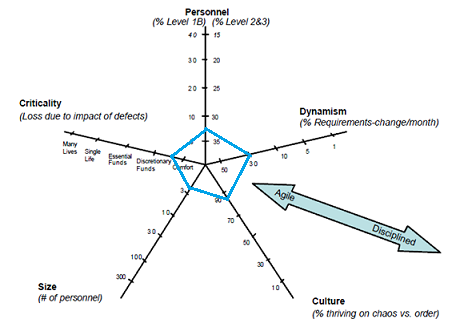
\includegraphics[width=0.75\textwidth]{star}
	\caption{Stjernemodellen}
	\label{fig:Stjernemodel}
\end{figure}

\textbf{Personnel:} P� denne akse vises hvor erfarent et udviklerteam er. Da ingen i gruppen har nogen s�rlig stor erhvervsm�ssig erfaring p� trods af, at vi har lidt kendskab til teknologierne fra skolen, er vores vurdering at den vil ligge mellem 0-35 og 10-30. Hvilket peger hen imod en agil metode.

\textbf{Dynamism:} Her bestemmes hvor dynamisk man har behov for at v�re. Efter de f�rste par m�der med EqualSums blev det hurtigt klart for os at der ville komme mange �ndringer undervejs. Mange kunder har sv�rt ved at s�tte ord p� hvad de egentlig gerne vil have til at starte med. Derudover er der flere forskellige vi snakker med som st�r for hvert deres omr�de. Det betyder vi ligger omkring de 30 som peger p� en rimelig agil metode.

\textbf{Culture:} Her ser man p� hvordan teamet trives bedst. Skal der v�re regler og procedure for alle, eller har man mere frihed til selv at v�lge. Vores team har det godt med et forholdsvist frit arbejdsmilj�. N�r vi ser p� EqualSums hvor vi laver programmet er der ogs� meget stor frihed og medarbejderne i virksomheden trives herunder. Derfor er det kun naturligt for os at ligger os t�t p� de 90 som igen peger p� en agil metode.

\textbf{Size:} Her kigger man p� hvor stort ens team er. Da vi arbejder i en lille to mandsgruppe er den nem at s�tte p�. Hvilket igen vil sige det ligger sig op af en agil metode. Store grupper kan blandt andet have sv�rt ved at kommunikere og koordinere et stort projekt hvor imod et lille hold nemmere kan styre hvem der laver hvad. 

\textbf{Criticality:} Criticality afg�res af hvor store konsekvenser fejl i systemet vil have. I vores system kommer fejl ikke til at have den store betydning. De kommer hverken til at koste menneskeliv eller vanvittige �konomiske nedture for firmaet. Derfor l�gger vi os ind mod midten igen og dermed en agil metode.

\subsection{Anbefalet metode valg}
Ud fra vores analyse i foreg�ende kapitel ved hj�lp af stjernemodellen, er det tydligt at se vi ligger os op af en agil metode. Som metode har vi valgt at bruge Scrum. Vi har allerede erfaring med Scrum fra vores andre projekter samt fra vores praktikophold. Vi syntes derfor scrum er et oplagt metodevalg til vores projekt. Der vil dog i projektet ogs� blive benyttet elementer fra andre metoder, da agil udvikling netop handler om at tilpasse arbejdsformen, alt efter behov. Vi har derfor valgt at tage nogle rutiner med fra nogen af de andre metoder. Fra UP har vi valgt at g�re brug af dom�nemodellen, samt vores databasediagram. Dette giver et godt fundament, is�r som mindre erfarne. Derudover har vi ogs� l�nt v�rkt�jerne, refactoring og testing som de prim�re fra XP, men ogs� pair programmering, f�lles kode og kodestandarder vil blive brugt. 

En af grundene til vi ikke har valgt at arbejde ud fra en UP metode, er blandt andet stjernemodellen, men i h�j grad ogs� vores korte projektperiode. Da vi har et meget begr�nset tidsrum til at f� lavet programmet, er der ganske enkelt ikke tid til at analysere s� meget. Derudover ligger det ogs� klart, at der kommer mange udvidelser til systemet da vi igen p� grund af den begr�nsede tid er blevet n�dsaget til at afgr�nse problemomr�det. Det vil sige, at der er mange opgaver vi slet ikke har med i dette opl�g, som skal laves bagefter.


\subsection{Scrum}
Scrum er en agil udviklingsmetode skabt tilbage i 90'eren. Det er et interaktivt og inkrementalt framework som hurtigt er blevet meget popul�rt blandt udviklere, da det giver en stor frihed, men samtidig s�tter nogle fast rammer for arbejdsgangen.

\subsubsection{Roller}
I Scrum vil man st�de p� rollerne Scrum Master, Produkt Owner og Scrum Team. Vores Produkt Owner er Martin Skov Kristensen og er salgschef hos Equalsums. Det er ham der st�r for projektet sammen med os, s� det var naturligt at give ham den rolle, som blandt andet indeb�rer at prioritere user stories og st� til r�dighed n�r der er sp�rgsm�l omkring produktet. Som Scrum master har vi valgt Peter. Valget faldt p� Peter fordi han havde erfaring med programmet ScrumDesk som vi bruger til at styre vores backlog, sprints, osv. Gregers er en del af selve Scrum teamet som udvikler. Peter indg�r selvf�lgelig ogs� som en del af teamet og udvikler sammen med Gregers.

\subsubsection{Strukturen}
Vi arbejder med 14 dags(10 arbejdsdage) sprints hvor vi har 2� arbejdsdag til udvikling p� systemet. Grunden til vi ikke har mere er, at der skal v�re tid til rapportskrivning. Vi har en velocity p� 0,7 hvilket betyder vi har 53,2 effektive timer til hvert sprint.
  
Da vi altid sidder ude i virksomheden n�r vi udvikler p� produktet, indg�r vi ogs� i deres Scrum holds daglige Scrum m�der, og hvis der ellers er nogen f�lles m�der. Internt i vi vores projekt holder vi ogs� et dagligt Scrum m�de, hvor vi kort fort�ller hvad vi har lavet og hvad vi har t�nkt os at g� i gang med n�ste gang. Derudover holder vi ogs� et sprint review m�de med Martin (produktowneren) hvor vi viser det frem vi har lavet i sprintet. Det g�r vi for at sikre at det vi har lavet lever op til Martins forventninger. Scrum retrospective holder vi l�bende dels fordi vi kun er to p� holdet og hele tiden snakker sammen under forl�bet, og dels fordi man har en tendens til at glemme hvad der gik d�rlig og is�r hvad gik godt.

\subsection{Tests}
For at sikre en h�j kvalitet i vores program har vi valgt at g�re brug af Unit Test, Integrationsest og til sidst Acceptance Test. Udover at v�re med til at h�jne kvaliteten i koden, sikrer disse tests ogs�, at koden virker, og rent faktisk g�r det den skal g�re. Der drages ogs� fordel ved at bruge de to f�rst n�vnte test n�r der laves refactoring. N�r der er blevet refactoret i koden er det nemt og hurtigt at teste om den stadig virker som den skal, ved at k�re disse tests.
Udover at hj�lpe udviklerne, giver det ogs� ejerne et gennemteste produkt, som vil v�re i h�jere kvalitet. 
\subsubsection{Unittests}
Der er valgt at unitteste enkelte metoder i systemet fremfor at bruge det som en test-dreven proces. Dette g�res, fordi den n�dvendige erfaring med at k�re et test-drevet projekt mangler, og derfor vil det bliver for stor en tidsr�ver.

Da der er gjort meget ud af at designe MVC arkitekturen s� systemer udviklet i dette er nemme at teste p�, har vi rig mulighed for at teste store dele af vores system. \citep{UnitTestMVC}

I systemet testes blandt andet om der modtages de rigtige Views, og om den medsendte ViewModel er korrekt. En ViewModel er data man sender til sit View, ofte vil det v�re en klasse, eller en IEnumerable. IEnumerable er et Interface der g�r det muligt at bruge et for-each loop p� vores collection af objekter. 

I forbindelse med at teste metoder i vores controller lag, er der implementeret et Repository Pattern, til at hj�lpe med at isolere Unit testene. Hvis man bruger den database man sidder og udvikler p� kan man ikke l�ngere stole p� disse resultateter. Dette skyldes, at indholdet af databasen kan blive �ndret i forbindelse med tests hvor der skrives til databasen. Derfor mocker man de data s� de altid er de samme, s� foruds�tningen for testen altid er den samme.
Repository Pattern og hvordan vi pr�cist bruger unit test i den forbindelse kan der l�ses mere om i et senere afsnit. 

N�r der er blevet refactoret en eller flere metoder er det hurtigt og nemt at teste om de forskellige Views og ViewModels stadig er rigtige. Derudover testes metoderne selvf�lgelig ogs�, s� man er sikker p� de stadig g�r det de skal, selvom de eventuelt er blevet skrevet om. Det sikrer os imod der pludselig er dele af systemet der ikke l�ngere virker.
 
\subsubsection{Integrationstests}
Udover unittests er der ogs� valgt at lave Integrationstests. Her testes flere dele af systemet sammen, for at sikre sig at de forskellige lag snakker ordenligt sammen.

I systemet er der lavet integration tests p� nogle User Stories, hvor der testes i GUI og hele vejen ned til DB-laget. P� den m�de bliver alle lagene testet fra top til bund. Her er det igen nemt at teste om en hel userstory stadig virker, hvis der for eksempel skulle komme �ndringer fra Produkt Owneren, s� man bliver n�dt til at refactor en eller flere af metoderne. 

\subsubsection{Acceptancetests}
Sidst vil der blive lavet en Acceptancetest sammen med Produkt Owner, og eventuelt nogen af brugerne p� systemet. Det g�res fordi det er kunden der bedst ved hvordan systemet skal virke og derfor er det en k�mpe hj�lp af f� dem til at teste systemet. P� den m�de er man sikker p�, at det lever op til deres forventninger.

\section{Teknologier}
N�r der skal udvikles web-applikationer, er der utroligt mange valg at tr�ffe rent teknologim�ssigt. Der skal tr�ffes valg for b�de backend, frontend, database og alt derimellem. Hvis der skal v�re fancy animationer skal der s� bruges html5 eller flash - eller silverlight? Skal backenden v�re php eller asp.net? Skal databasen v�re en postgresql, mssql eller mysql-database? Hvordan snakker backend og frontend sammen? xml, json eller noget helt tredje? Der er mange muligheder og i det f�lgende kapitel bliver de valg vi har truffet forklaret og begrundet.

\subsection{MVC}
Overordnet set har vi valgt at arbejde med \emph{Microsofts ASP.net mvc3 framework}. Dette giver en logisk opbygning i projektet, der bliver delt op i \emph{Model}, \emph{View} og \emph{Controller}. Udover, at det holder sig t�t op af den 3-lags arkitektur som vi har brugt i uddannelsen, giver det ogs� �get overblik. Samtidig giver det mulighed for at bruge \emph{Microsofts Razor View Engine} \citep{razor} (Herefter blot Razor) der i forhold til tidligere l�sninger som f.eks. web forms giver �get l�sbarhed og enklere syntaks.
\subsection{Database}
\subsubsection{EntityFramework}
I Equalsums bruges Devarts entity framework (Herefter EF) til at forest� kommunikation mellem database og backend. Da EF ud fra databasen selv konstruerer modeller er det en v�sentlig forenkling i forhold til at bruge sql-s�tninger. 

I al sin enkelthed fort�ller man EF, at man f.eks. gerne vil have fat i en kunde-objekt fra databasen, og herefter vil EF selv finde ud af, hvilke relationer der findes i databasen, og s�rge for at hente al relevant data ud. Det samme g�r sig g�ldende ved inds�tning, hvor man laver et objekt med de �nskede attributter, og herefter fort�ller EF at det skal gemmes i databasen, hvorefter de enkelte v�rdier bliver indsat i de forskellige tabeller med de rette relationer. Med andre ord, EF s�rger selv for at foretage mapning mellem databaserelationer, og derudfra dannes et s�t af objekter. P� denne m�de undg�r man, at skulle lave lange, komplicerede join-s�tninger. S�fremt fremmedn�gler og prim�rn�gler er korrekt definerede, kan alt dette overlades til EF. 
\subsubsection{LINQ}
LINQ \marginpar{\textbf{L}anguage \textbf{IN}tegrated \textbf{Q}uery} er som s�dan ikke specifikt til brug for databaser, men da det er til at lave vores database-queries vi bruger LINQ, vil det blive n�vnt i database-afsnittet.

LINQ udm�rker sig ved at lave sql-lignende kald. Forskellen er, at man kan bruge LINQ p� andre datakilder end databaser, f.eks. arrays. LINQ g�r brug af \emph{anonyme typer} og \emph{lambda-expressions} - disse er typer og funktioner der oprettes ad hoc, det vil sige, at de kun eksisterer s� l�nge de bruges, og man undg�r derved, at oprette en m�ngde klasser og metoder. I det f�lgende eksempel vises et linq-udtryk, hvor man i en graf vil have alle ikke-bes�gte noder:

\begin{figure}[H]
\lstset{language = CSharp}
\begin{lstlisting}
var unvisitedNoteList = (select from n in nodeList
																where n.visited == false
																select n);
\end{lstlisting}
\caption{LINQ-kald der henter en liste af nodes}
\label{fig: LINQ_first}
\end{figure}

En foresp�rgsel af denne type, ville resultere i en IEnumerable der indeholdt node-objekter (hvor egenskaben visited er falsk).

Man kan ogs� lave sine egne objekter, hvis man �nsker at hente specielle objekter. Dette vil blive yderligere uddybet p� side \pageref{json} under "JSON".

\subsubsection{Open Authorization (oAuth)}
Open Authorization eller oAuth, er en standard for autorisering af f.eks. websiders brug af brugerkonti, uden at brugeren skal udlevere brugernavn og password. oAuth giver ganske enkelt en applikation adgang til en brugers konti uden at applikationen kender brugernavn og password. 

F�r denne forklaring, vil et par termer blive pr�ciseret:
\begin{description}
\item[Bruger]
Brugeren er ejeren af kontoen der skal tilg�s, brugeren kender sit brugernavn og password.

\item[Klient]
Klienten er det program eller den side der skal tilg� brugerens konto. Klienten m� ikke kende brugerens password.

\item[Server] 
Serveren er den entitet der holder styr p� brugerens konto, og hvem der har adgang til den, serveren ved hvorn�r brugerens password er rigtigt\footnote{Det er d�rlig skik at opbevare brugerens password i klar-tekst, et hash af brugerens password er at foretr�kke}.
\end{description}

Grundl�ggende findes der to former for oAuth: 2-legged og 3-legged. Disse to former vil ganske kort blive forklaret, hvorefter det valg der er foretaget i forbindelse med dette projekt vil blive begrundet.

\textbf{3-legged Authorization}
Klienten sender en foresp�rgsel til serveren og modtager en usigneret access token, samtidig sendes brugeren videre til Serveren. Brugeren identificerer sig overfor serveren, hvorefter klienten modtager en signeret token, som er g�ldende for den specifikke session. Denne token sendes til klienten. Klienten kan nu bruge denne token til at signere fremtidige requests, og derved identificere sig over for serveren, som godkendt. Der er alts� tre parter i denne transaktion, bruger, klient og server \citep{reilly}.

\textbf{2-legged Authorization}
2-legged authentication bruges hvor brugeren ikke kan identificere sig over for serveren ved starten af hver session. Det kan f.eks. v�re ved brug af applikationer p� en mobil enhed. Istedet opretter brugeren en hemmelig n�gle, for hver klient. Klienten kender denne hemmelige n�gle og bruger den til at danne en access token, som bruges til at identificere sig som en af brugeren godkendt klient. I denne transaktion er der kun to parter, klient og server.

Klienten f�r adgang uden, at brugeren fort�ller klienten sit password. Samtidig kan brugeren s�tte regler for hvilke rettigheder den enkelte klient har. Dette kendes is�r fra Facebook, hvor applikationer skal bede om specifikke tilladelser til f.eks. at skrive p� brugerens v�g, l�se vennelisten osv.
 
Vi vil i projektet benytte 2-legged authentication til at tilg� Googles api p� vegne af brugeren. Vi kunne have valgt at bruge 3-legged, da denne er velegnet til brug ved websider, men da man skal identificere sig hver gang man starter en ny session (har haft browseren lukket), blev det vurderet, at det ville blive et irritationsmoment. Samtidig bruger EqualSums Google apps, hvilket muligg�r 2-legged authentication. Vi valgte derfor 2-legged authentication, da det for brugeren tilbyder en langt smidigere login-oplevelse.

\subsubsection{Google api}
Google tilbyder api til stort set alle services, hvadenten det er maps, docs, calendar, mail eller noget helt andet. Projektet skal autentificere sig via 2-step authentification, og heldigvis har Google lavet et .net library der tilbyder b�de 2- og 3-step authentication.


\subsection{Frontend}
Det har altid v�ret forbundet med stort besv�r at udvikle hjemmesider der ser ens ud, og opf�rer sig ens i alle browsere. Dette skyldes at der findes en lang r�kke standarder, og at alle browsere underst�tter disse standarder i st�rre eller mindre grad. Det har derfor v�ret n�dvendigt at benytte sig af workarounds og hacks, der udnytter de forskellige browseres svagheder og styrker. 

I vores arbejde slipper vi for denne problemstilling, da systemet der udvikles, kun skal bruges internt. Eftersom EqualSums udelukkende bruger Google Chrome, er det kun n�dvendigt at udvikle til en enkelt browser. I det efterf�lgende vil brugen af forskellige front-end teknologier blive forklaret.

\subsubsection{Razor View Engine}
Som tidligere n�vnt bruger vi Microsofts Razor View Engine, der er en ny view engine til asp.net. Fordelen ved at bruge Razor er, at der er en kraftigt forenklet syntaks. Samtidig er Razor smart nok til, selv at vide, hvorn�r der er tale om et @ der starter en blok, og hvorn�r det er @ i en e-mail adresse. Dette betyder ogs�, at man ikke beh�ver markere n�r en razor-blok afsluttes, til forskel fra asp hvor man bruger \%$>$ og php hvor man bruger ?$>$. N�r man starter en Razor kodeblok skriver man ganske enkelt @ efterfulgt at koden. Det er her vigtigt at huske, at der ikke skal semikolon efter blokken. 

Dette �ger l�sbarheden af koden, og hastigheden hvormed man udvikler, da det er langt mere intuitivt.

\subsubsection{jQuery}
jQuery er et framework til javascript der virker i alle moderne browsere, og man skal som udvikler ikke bekymre sig om browser kompatibilitet. Grundideen bag jQuery er "Write less, do more". Som eksempel kan n�vnes, at man har mulighed for at bruge css-selectorer (og pseudoselectorer) til at v�lge elementer. Man slipper derfor for at bruge document.getElementById og andre m�rkelige konstruktioner, da man kan gribe direkte ned i DOM-tr�et\marginpar{\textbf{D}ocument\\\textbf{O}bject\\\textbf{M}odel}\footnote{Den grundl�ggende opbygning af et html-dokument}. Man kan f.eks. v�lge den f�rste r�kke i tabellen med id "customers" ved at skrive 

\lstset{language = javascript}
\begin{lstlisting}
$("\#customers:first-child") 
\end{lstlisting}

Udover det er meget nemmer at v�lge et bestemt element, er det ogs� nemt at manipulere elementerne uanset, om man vil �ndre, tilf�je eller fjerne indhold, tekst, css-egenskaber eller v�rdier.

Denne fleksibilitet sammen med en lang r�kke indbyggede funktioner til animationer g�r jQuery til et effektivt redskab, n�r der skal bruges Javascript p� en side. Desuden g�r jQuerys popularitet, at der findes en lang r�kke plugins, som tilf�jer n�sten enhver funktionalitet man kan t�nke sig.

\subsubsection{AJAX}
I forbindelse med kommunikation mellem front-end og backend vil vi i h�j grad benytte \marginpar{\textbf{A}synchronous \textbf{J}avascript \textbf{A}nd\\ \textbf{X}ML} AJAX, som muligg�r asynkron kommunikation mellem klient og server. Dette betyder, at der kan hentes og sendes data uden, at siden skal refreshes. P� den m�de f�r brugeren en langt bedre og flydende oplevelse, end hvis der skulle refreshes hver gang klienten skulle sende eller foresp�rge data fra serveren. Dette er med til at h�jne brugervenligheden.

Et sted hvor man bruger AJAX, er ved autofuldf�relse, som f.eks. kendt fra Google-s�gninger. Har man en debugger der overv�ger serverrequests, som f.eks. Firebug mens man skriver sin s�gning, vil man se, at der bliver sendt en request for hvert tastetryk. Dette er AJAX-requests der bliver sendt.

Netop brugen af jQuery g�r det langt nemmere at benytte sig af asynkrone kald, idet der i jQuery findes en indbygget funktion til at sende asynkrone foresp�rgsler til serveren, der forenkler processen, som det ses i figur \ref{fig: jQuery}


\begin{figure}[H]
\lstset{language = javascript}
\begin{lstlisting}
var data = {userId: 4}
var url = {"CRMsystem/feedDetails/getUserName"}

$.getJSON{url, data, function(data){
	$("#customerName").text(data);
}
\end{lstlisting}
\caption{Asynkront jQuery-kald}
\label{fig: jQuery}
\end{figure}
\subsubsection{JSON} \label{json}
\marginpar{\textbf{J}ava\textbf{S}cript \textbf{O}bject \textbf{N}otation}
Vi har dog valgt at benytte JSON istedet for XML som dataformat til AJAX-requests. F�rst og fremmest skyldes dette, at JSON er lavet specielt til Javascript, men samtidig er der langt mindre data der skal sendes frem og tilbage, da data ikke skal markeres p� samme m�de som XML hvorved der er langt mindre overhead:
\begin{figure}[H]
\lstset{language = xml}
\begin{lstlisting}
<?xml version="1.0" encoding="UTF-8"?>
<persons>
	<person>
		<firstName>Thomas</firstName>
		<lastName>Hansen</lastName>
		<address>Guldvej 23</address>
		<city>Aalborg</city>
		<zipCode>9000</zipCode>
		<email>thomas@gmail.com</email>
	</person>
</persons>

\end{lstlisting}
\caption{XML-eksempel}
\label{fig: bigXml}

\end{figure}
\lstset{language=javascript}

\begin{figure}[H]
\begin{lstlisting}
person[
	{
		firstName: "Thomas", 
		lastName:"Hansen", 
		address: "Guldvej 23", 
		city: "Aalborg", 
		zipCode: 9000, 
		email:"thomas@gmail.com"
	}
]

\end{lstlisting}
\caption{JSON-eksempel}
\label{fig: bigJson}

\end{figure}
Som det ses af figur \ref{fig: bigXml} og \ref{fig: bigJson}  er JSON-objekter langt enklere end XML-objekter, i det viste eksempel er der tale om et array (omgivet af []) med et enkelt objekt. Et objekt er omkranset af \{ og \}. 

At JSON er simpelt, er b�de en fordel og en ulempe. N�r der skal sendes data fra serveren til klienten, kan man ikke bare tage et objekt der er hentet fra databasen og serialisere det som JSON. Der opst�r problemer i forbindelse med cirkul�re referencer. Dette skyldes en begr�nsning i EF som Microsoft er opm�rksomme p� \citep{circRef}. Indtil der foreligger en l�sning, skal der benyttes en workaround, hvor man laver sine egne, speciallavede objekter via projection selector'en $select$ \citep[pp. 75-80]{rattz2010pro}. Eksemplet i figur \ref{fig: LINQ_second} tager udgangspunkt i fig. \ref{fig: LINQ_first}:

\begin{figure}[H]
\lstset{language = CSharp}
\begin{lstlisting}
var unvisitedNoteList = (select from n in nodeList
																where n.visited == false
																select new {
																	name = n.name,
																	value = n.value,
																	visited = visited
																});
\end{lstlisting}
\caption{LINQ-kald der henter en liste af nodes, der er klar til JSON}
\label{fig: LINQ_second}
\end{figure}

Med dette kald f�r man et objekt der indeholder egenskaberne name, value og visited. Denne brug af projektion-keyword'et select betyder, at de anonyme objekter serialiseres bagefter.

\subsubsection{CSS3}
Brugen af CSS3 giver en lang r�kke muligheder for at lave langt mere elegant design, her kan bl.a. n�vnes brug af gradienter og afrundede hj�rner. CSS3 er endnu ikke underst�ttet af alle browsere, og ved visse egenskaber (som f.eks. border-radius), skal der benyttes en egenskab for hver af de 3 browser-engines (Webkit, Mozilla og IE). Som tidligere n�vnt bliver der ikke problemer med cross-browser kompatibilitet.

\subsection{Versionstyring - SVN}
Til versionsstyring har benyttet SubVersion (SVN). Det er et open source system som ogs� benyttes hos EqualSums, s� det var meget naturligt at g�re brug af det ogs�. Det er et utroligt vigtigt redskab til at styre sin sourcekode. 

Hos EqualSums har vi en server hvor vores repository ligger med koden p�. Man kan s� lave et checkout med TortoiseSVN, hvilket betyder man f�r en lokal kopi. N�r man har lavet nogen �ndringer i koden, kan man commit det igen til sit repository, hvor det s� vil bliver merged med de eksisterende filer. P� den m�de har alle altid adgang til den nyeste kode. Skulle der bliver uploadet noget kode som man fortryder kan man lave en roll back til en tidligere revision.


\chapter{Arkitektur}
For at hj�lpe med at give et bedre overblik over systemet og hvordan de forskellige lag snakker sammen i forhold til hinanden, vil arkitekturen blive beskrevet her. 

\section{Arkitektur}

Da vi bruger MVC 3 har vi en stor del af vores grundstruktur. MVC som st�r for Model, View, Controll er ogs� delt op i netop disse tre lag. 

\begin{figure}[H]
	\centering
		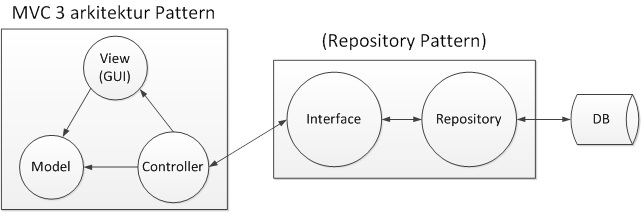
\includegraphics[width=1.00\textwidth]{arkitektur.jpg}
	\caption{Arkitektur}
	\label{fig:arkitektur}
\end{figure}

Som det kan ses p� figur \ref{fig:arkitektur} er MVC kun en del af arkitekturen. Der er implementeret et Repository pattern, for at opn� en r�kke fordele, som vil blive beskrevet i et senere afsnit. MVC controlleren st�r for at skrive til de klasser der er implementeret af repository pattern. Controlleren vil sende et objekt ned til sit repository, som skriver det til databasen. Det skal ses som et data access lag, det er her alt kontakt med databasen starter og stopper. Vores repositories vil hedde CompanyRepository.cs mens interfacet til denne vil hedde ICompanyRepository.cs. Navnet fort�ller selvf�lgelig noget omkring hvilket omr�de dette repository bruges.

P� figur \ref{fig:arkitektur} ses cirkelen kaldet Model. Det er vores klassiske modellag som man ogs� kender det fra 3-lags arkitekturen. Det er i dette lag dom�nemodellen bliver realiseret. Da der bruges Entity Framework styrer dette framework laget for os, og det vil derfor virke tomt. Der benyttes Database First tilgangen til at modellere laget ud fra designet af databasen. Derved bruges Entity Frameworket det meste af tiden til at styre dette lag. Vi laver dog nogle modelklasser manuelt s� som wrapper-klasser, eller ViewModels. Disse kunne blandt andet bruges hvis man vil sende to entity klasser til samme view. Eller har brug for nogle flere properties, som man ikke er interesseret i bliver gemt i databasen. Der vil komme eksempler p� disse senere i rapporten.

View p� figur \ref{fig:arkitektur}, er det grafiske interface, som st�r for at vise den HTML brugeren skal se. Et View benyttes ofte sammen med en model. Det vil sige et objekt med en r�kke properties som man �nsker vist i viewet. Det kunne v�re et Company objekt der bliver sendt som model, hvor efter viewet har adgang til dens properties. Her er ogs� mulighed for at bruge IEnumerables hvis det er lister man vil skrive ud. Hvis man har en web-form p� siden er det muligt at sende samme type objekt tilbage til controlleren, med alle de nye properties man har sat i web-formen. Et view vil ligge en mappe af samme navn som den controller den h�re til. De vil typisk have et navn der forklare indholdet af siden, f.eks. Company.cshtml.

Normalt er det meningen, at view- og modellaget er skarpt adskilt af controllerlaget, s� model og view aldrig kommunikerer direkte. Frameworket er dog skruet s�dan sammen, at controlleren sender et model-objekt direkte til viewet. 

Controller p� figur \ref{fig:arkitektur} er vores controllerlag. Controlleren styrer hvad der sker i applikationen, og st�r for at f� vist de rigtige views. Den vil minde meget om det controllerlag man ogs� ser i 3-lags arkitekturen. Det er her vi modtager input fra brugeren og opretter objekter som vi sender videre ned til vores data access lag. (Repository pattern). Alle controllere hedder Controller til sidst. Alts� en controller til at styre sine companies ville oplagt hedde CompanyController.cs. Dette er bestemt af MVC 3. 

Selve mappe- og filstrukturen bliver selvf�lgelig i h�j grad bestemt af MVC, men for at g�re overblikket af systemet totalt vil vi kort beskrive strukturen her.

\begin{figure}[H]
	\centering
		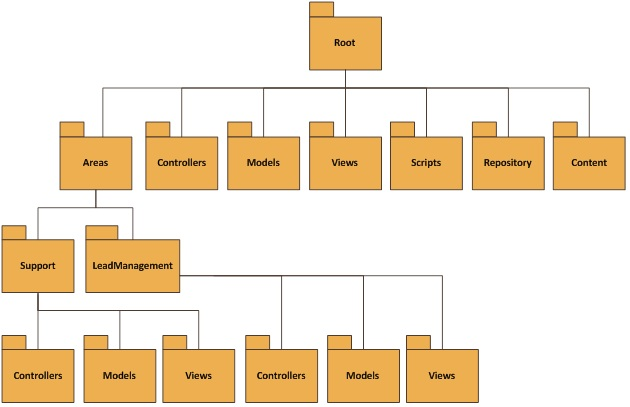
\includegraphics[width=1.00\textwidth]{mappestruktur.jpg}
	\caption{Mappestruktur}
	\label{fig:Mappestruktur}
\end{figure}

I roden af projektet vil man finde nogle config filer med forskellige ops�tninger af sitet. Blandt andet SQL forbindelse. Der udover bruges Content til alle CSS filerne, Scripts til JavaScript og jQuery frameworket. I Repository ligger repository klasserne samt deres interface. Controllers, Models og Views er MVCs struktur, og burde v�re selvforklarende. Mere interessant er Areas \citep[pp. 374-381]{freeman2011pro} som er MVCs m�de at lave sub-directories p�. Hver mappe i et Area f�r nemlig hver sin Controllers, Models og Views mappe som virker p� samme m�de som dem i Root mappen. Det g�r det nemt at flytte en del af systemet ud i et sub-directory, da alt vil opf�re sig p� samme m�de s�fremt det ligger i samme sub-directory.

\chapter{Teori}
\section{Patterns}

Som n�vnt i forordet p� s. \pageref{quote}, kan patterns beskrives som generelle l�sninger, der har vist sig at virke p� mange problemer. Patterns er alts� en form for "altmuligv�rkt�jer" som en programm�r kan benytte sig af. 

\subsection{Form�l}
Form�let, eller ideen med patterns er, at det er l�sninger, der kan bruges i mange tilf�lde. P� denne m�de undg�r programm�rer at skulle opfinde den dybe tallerken igen og igen. Samtidig er patterns den bevist bedste m�de at l�se problemerne p�, s� man undg�r fejl, s�fremt patterns'ne implementeres korrekt. 

I det f�lgende vil vi forevise en r�kke patterns, som vi har brugt i arbejdet med CRM-systemet. Vi vil gennemg� hvilke former for problemer de l�ser, hvordan de implementeres, og hvordan og hvorfor vi har benyttet os af dem. Vi har dog valgt at se bort fra helt simple patterns som f.eks. singleton.

\subsection{Forskellige patterns}
\subsubsection{Repository}
Repository pattern er en m�de at adskille kommunikationen mellem databasen og resten af programmet. Det er her vi skriver og l�ser til og fra databasen. Det skal sammenlignes med et data-accesslag. N�r der i dette afsnit tales om repository er det i forhold til Repository pattern, som ikke m� forveksles med database repositories.

Ved at implementere repository pattern undg�s blandt andet en masse kodeduplikation idet vi kalder ned til vores repository hver gang og genbruger p� den m�de de forskellige metoder. 

Udover mere abstraktion i designet, giver det ogs� mulighed for bedre at kunne unit teste systemet. Det hj�lper med at isolere de metoder der skal testes, ved at g�re det langt nemmere at forfalske (Mock) vores data. 

\subsubsection{Implementering af Repository}
M�den repository'et er implementeret p�, er med henblik p� at kunne unit teste med et testing framework kaldet Moq \citep{Moq}, dette ogs� giver samtidig den �nskede abstraktion. For at hj�lpe med at danne et overblik over vores implementering har vi lavet f�lgende diagram. 
\begin{figure}[H]
	\centering
		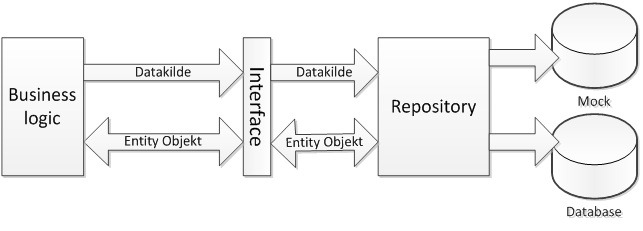
\includegraphics[width=0.75\textwidth]{repositorymodel}
	\caption{Respositorymodel}
	\label{fig:Respository}
\end{figure} 
Som det ses her, har vi vores forrentningslogik f�rst. Her bestemmes hvilken datakilde der skal bruges. Dette vil afh�nge af, om vi kommer fra f.eks. en unit test med Mocked data, eller hvis det er en Integrations test som vil bruge de virkelige data til at teste p�, eller hvis vi selvf�lgelig bare bruger programmet normalt. Dern�st har vi vores interface, som f�re os videre ned i vores repository som s� henter den �nskede data fra den �nskede datakilde.

Vi startede med at lave et repository lag i vores projekt. Her opretter vi alle vores repository klasser samt deres interface klasser. Se evt. afsnittet om arkitekturen. N�sten alle vores MVC controllere har hvert sit repository da controllerne n�sten altid d�kker et bestemt omr�de i database. Hvis dette ikke er tilf�ldet genbruger man selvf�lgelig det repository som har de n�dvendige metoder. P� den m�de kan vi ogs� genbruge mange af vores metoder i vores repositories. 

Vores repository implementere selvf�lgelig det interface der h�rer sig til. Derudover har vi en constructor hvor vi s�tter hvilken datakilde den skal bruge. Da vi bruger Moq kan vi mock dette s� den eksempelvis opfatter en simpel tabel som datakilde. Dybere forklaring omkring dette kommer senere i afsnittet.

\begin{figure}[H]
\lstset{language = CSharp}
\begin{lstlisting}
public class ContactRepository : IContactRepository
{
    private CRMSystemEntities _db;
    public ContactRepository(CRMSystemEntities repository)
    {
        _db = repository;
    }
}
\end{lstlisting}
\caption{Repository Constructor.}
\label{fig: rep_Constructor}
\end{figure}

I selve respositoriet vil der selvf�lgelig v�re en implementering af hver enkel metode angivet i interfacet, disse er undladt her, da de ikke er relevante.

Da det er vores controllere der st�r for at styre hvilken datakilde der skal g�res brug af, har vi oprettet en r�kke contructors til netop at styre dette.

\begin{figure}[H]
\lstset{language = CSharp}
\begin{lstlisting}
public class LeadDetailsController : Controller
    {
        private IContactRepository _repo;

        public LeadDetailsController()
        {
            this._repo = new ContactRepository(new CRMSystemEntities());
        }
        
        public LeadDetailsController(IContactRepository repo)
        {
            this._repo = repo;
        }
        
        public LeadDetailsController(CRMSystemEntities db)
        {
            this._repo = new ContactRepository(db);
        }

        public IContactRepository LeadDetailsRepository
        {
            get { return _repo; }
        }
   }
\end{lstlisting}
\caption{Controller Constructor.}
\label{fig: con_Constructor}
\end{figure}

Den f�rste constructor bruges n�r der eksempelvis skal hentes eller sendes data fra et View som samme controller styrer. Den bruger vores entity framework som standard.
Efter den har vi den constructor vi bruger, n�r vi mocker vores datakilde til Unit Tests. Som det kan ses tager den et interface som parameter. Det er det object vi mocker i vores unit test.

Den sidste bruges hvis dette repository skal bruges fra en anden controller. I Entity frameworket er objekter bundet til en bestemt context, s� for at kunne sende objekterne igennem controlleren skal vi have den context med som de er bundet til. Det er det vi g�r med denne constructor. Derudover har vi en simpel property for at kunne f� fat i repositoriet fra andre controllere.
\subsubsection{Unit Test med repository}
(Denne unit test h�rer til en anden MVC controller og repository end de forg�ende eksempler)
Her vil vi kort beskrive en test metode, for at vise hvordan vi benytter repository pattern i forbindelse med unit testing.

\begin{figure}[H]
\lstset{language = CSharp}
\begin{lstlisting}
[TestMethod()]       
public void BugDetailsTest()
{             
    Ticket[] ticketss = new Ticket[] {
        new Ticket() {Ticketsid = 1, Headline = "test1", Content = "bla",... },
        new Ticket() {Ticketsid = 2, Headline = "test2", Content = "blabla",... },
        new Ticket() {Ticketsid = 3, Headline = "test3", Content = "blablabla",... }
    };
    int id = 2;            
    Mock<ITicketRepository> mock = new Mock<ITicketRepository>();
    mock.Setup(m => m.GetDetails(id)).Returns(ticketss[id - 1]);
            
    TicketController target = new TicketController(mock.Object);
    var result2 = target.BugDetails(id) as ViewResult;
    Ticket ticket = (Ticket)result2.ViewData.Model;

    Assert.AreEqual("blabla", ticket.Content);
}
\end{lstlisting}
\caption{Unit Test.}
\label{fig: UnitTest}
\end{figure}

Testen er en standard unit test der f�lger den typiske "arrange, act, assert". Der startes med at lave et array af Tickets som her vil blive datakilden. Dern�st lavers et mock af ITicketRepository. Derudover laves en instans af TicketController hvor der bruges den contructor der tager imod et ITicketRepository objekt som parameter. P� den m�de ved testen, at vi vil benytte vores array af Tickets som datakilde. Til sidst tjekkes det om det er den forventede data der returneres. 

\subsubsection{Decorator}

I og med, at der skulle laves et dynamisk filter, hvor det p� forh�nd ikke var vidst hvilke parametre der skulle filtreres p�, var det n�dvendigt at finde en l�sning der gav en vis grad af fleksibilitet.

Problemet med at bruge Entity framework og LINQ er, at det ikke er muligt at lave dynamiske queries p� samme m�de som i sql. Dette er n�dvendigt i forbindelse med filter-funktionen, da det p� forh�nd ikke kan siges, hvilke kategorier der skal sorteres p�, og hvordan. I SQL kan man f.eks. tilf�je en streng til sin query, som er baseret p� andre variabler:

\verb|string completeQuery = query +" AND WHERE userId > 23 " + sortPart;|

Det er ikke muligt p� samme m�de at tilf�je eksempelvis betingelser i LINQ-kald.

 Normalt bruges Decorator pattern til at tilf�je funktionalitet til en klasse. Et decorator pattern fungerer ved, at man har en ConcreteComponent, som decoratorklassen arver fra. Decoratorklassen er den klasse som skal dekoreres. Den initialiseere, hvorefter man giver den videre til en anden klasse som parameter. Denne nye klasse tilf�jer s� funktionalitet, og den nye klasse bliver s� igen givet videre til en anden klasse osv. Denne senden klasser videre, bliver gjort mulig via et factory pattern. Et decorator pattern vil is�r typisk blive brugt ved grafik, hvor man f.eks. kan tilf�je funktionalitet som scrollable, resizable osv til et vindue, hvor vinduet et grundklassen.

\begin{figure}[H]
	\centering
		
\includegraphics[width=0.55\textwidth]{Decorator}
	\caption{Decorator Model}
	\label{fig:Decorator}
\end{figure} 

P� modellen kan ses "grundklassen" (concreteComponent) og dekorat�ren, som er den klasse der skal dekoreres. �verst ses interfacet Component, som er det interface decorator'en arver fra. 

\textbf{Implementering}


\label{chap: decorator}
M�den vi implementerede decorator-pattern'et p�, var ved at f�rst lave en generel abstrakt klasse "ConcreteQuery". Denne klasse indeholder ganske simpelt en liste over companies samt en metode "DoQuery()". Herudover, er der ogs� en constructor, der tager generelle parametre, og l�gger dem i de relevante properties. Desuden lavede vi en klasse for hver kolonne i oversigten, som s� kan kaldes og filtrere resultaterne.

Hver klasse har en constructor der tager imod det FilterItem der h�rer til dem, og samtidig tager imod Company-listen som den ser ud pt. Herefter bliver filteret p�f�rt listen, og listen returneres.
  \\
\begin{table}[H]
\centering
\begin{tabular}{|ll|}

  \hline
		\multicolumn{2}{|c|}{FilterItem} \\
		\hline
		Values & List$<$string$>$\\
		Criteria & List$<$int$>$\\
		CompanyList& List$<$Company$>$\\
		Type& string\\
		Category &string		\\
		\hline
		
		\end{tabular}
	\caption{Attributter for FilterItem-klassen}
	\label{fig:FilterItemModel}
\end{table}


\begin{figure}[H]
	\caption{city-query klassen, l�g m�rke til der arves fra concretreQuery og, at den constructor kaldes}
	\label{fig: cityQuery}
	\lstset{language = CSharp}
	\begin{lstlisting}
public class CityQuery : ConcreteQuery
{
    public CityQuery(List<CompanyViewModel> companyList, List<string> values, int criteria)
        : base(companyList, values, criteria)
    {
        companyList = (from c in companyList
                       where c.Company.City != null
                       select c).ToList();
    }

    public override List<CompanyViewModel> DoQuery()
    {
        List<CompanyViewModel> returnList = new List<CompanyViewModel>();
        string value = values[0];
        if (this.criteria == 1)
            returnList = (from c in companyList
                          where c.Company.City.Cityname.ToLower().Contains(value.ToLower())
                          select c).ToList();
        else
            returnList = (from c in companyList
                          where !c.Company.City.Cityname.ToLower().Contains(value.ToLower())
                          select c).ToList();

        return returnList;
    }
}	
\end{lstlisting}
\end{figure}

Som det ses af kodeeksemplet i figur \ref{fig: cityQuery}, kan man se, at vi har en f�lles constructor der bliver arvet fra ConcreteConstructor, denne constructor bliver kaldt og modtager kriterie og v�rdi fra det respektive FilterItem-objekt. Disse gemmes under de relevante egenskaber. Herefter tager query-klassen over, og behandler data hvis det er n�dvendigt, f.eks. hvis der er tale om tal-data, bliver de konverteret fra en string til integer. 

Det er forholdsvist simpelt n�r vi benytter filteret. Filtercontrolleren f�r tilsendt en liste med filterItems. Som det ses p� figur \ref{fig:FilterItemModel} er FilterItem ikke andet end en beholder der holder v�rdier der er relevate for et enkelt filter.

Herefter l�bes listen af filtre igennem, og den dertilh�rende query h�ftes p� concreteQuery-klassen via klassen QueryFactory. Resultatet heraf returneres til controlleren, controlleren serialiserer herefter listen til JSON og sender den tilbage til klienten.



\chapter{Produkt}
\section{Kravspecifikation}
EqualSums har stille en opgave der omhandler udvikling af et CRM system. Det de prim�rt var interesseret i at f� udviklet var deres h�ndtering af kunder. Hvor fokus ville v�re den m�de salgsafdelingen h�ndtere kunderne p�. Da det kun var en lille del af programmet vi skulle lave, blev der stillet krav om at programmet nemt skulle kunne udvides og vedligeholdes.
 
Selve produktet skulle kunne vise og h�ndtere alle firmaets kunder, og potentielle kunder. Der skal kunne laves aftaler med de forskellige leads, som ogs� bliver noteret i s�lgernes Google-kalender. Derudover skal der v�re mulighed for at skrive noter p� en lang r�kke af de data der er i systemet. Der blev ogs� stillet krav om at kunne sende mails direkte fra programmet, samt hente gamle mails frem.

Det de i bund og grund �nskede, var en effektiviseret kopi af det Google docs regneark de bruger nu, hvor man samtidig har styr over hvad man pr�cist har aftalt og har haft aftalt med kunderne.

Systemet vil overordnet indeholde tre sider, Min side, Leads Oversigt og leads detajler. I det f�lgende vil det kort blive forklaret hvilke opgaver det t�nkes der skal l�ses p� hver af de tre sider:

\subsubsection{"Min Side"}
Min Side vil v�re en oversigts side, hvor man har vist sin kalender, en liste over dagens g�rem�l. Det vil v�re her man starter p� n�r man er logget ind for hurtigt at kunne danne sig et overblik over hvad der skal laves i l�bet af dagen.
\begin{itemize}
	\item Der skal v�re en oversigt over dagens opgaver, for at g�re det hurtigt og nemt at overskue de opgaver man har for dagen
	\item Mulighed for at fjerne en opgave n�r den er l�st, s� man ikke l�ngere skal se og t�nke p� den
	\item Medarbejderens kalender skal vises p� siden s� man hurtigt og nemt kan se hvilken aftaler man har i l�bet af m�neden, og dermed ogs� nemmere kan planl�gge nye aftaler
	\item Man skal kunne se detaljer for dagens opgaver s� man kan f� en mere pr�cis beskrivelse af hvad der skal laves
	\item Sortere dagens opgaver s� man bedre kan styre hvilken r�kkef�lge man vil lave dem i
\end{itemize}


\subsubsection{"Leads Oversigt"}
Leads Oversigt er en stor tabel over alle de Leads der er i systemet. Her vil v�re forskellige sorterings muligheder for at kunne finde frem til de leads man vil arbejde med. Tabellen vil vise de vigtigste informationer omkring leadet, s� man nemt og hurtigt kan finde den information man er ude efter. Det er ogs� her man kan oprette nye leads, enkeltvis eller via en kommasepareret fil (.CSV). 
\begin{itemize}
	\item Der skal v�re en oversigt over alle Leads, s� man nemt kan finde de leads man har i systemet og l�se deres vigtigste data
	\item Mulighed for at sortere leads efter de viste data s� man kan f� en liste over pr�cis de leads man �nsker at arbejde med
	\item Man skal kunne opdatere data p� leads, s� de stemmer overens med virkeligheden
	\item Der skal v�re mulighed for at afm�rke flere leads og opdatere samme felt p� dem p� �n gang, s� man slipper for at skulle rette det samme data p� mange forskellige leads
	\item Der skal kunne uploades en CSV fil, med en masse leads s� man slipper for at skulle indtaste disse en ad gangen. Der skal samtidig tjekkes for dubletter s� man ikke f�r 	de samme leads flere gange
	\item Der skal v�re en blank plads i bunden s� man manuelt kan oprette et enkelt lead
	\item Skal kunne tilf�je en ny kolonne dynamisk i oversigten, s� man dynamisk kan tilf�je flere data at sortere efter
\end{itemize}


\subsubsection{"Lead Detaljer"}
Lead Detaljer indeholder en simpel liste af leads til venstre hvor der vil v�re nogle f� sorterings muligheder. Der kan v�lges leads ud fra denne liste s� man kan f� vist alle deres stamdata. Her vil ogs� v�re mulighed for at se hvilken kontakter man har med leadet.(Kontaktpersoner). Der vil der ogs� v�re mulighed for at se alle de aftaler man har lavet med dem. Det kan v�re m�der, telefon m�der, kurser etc. Her vil der evt. ogs� v�re vedh�ftet en note som man ogs� kan hente frem. Derudover vil der ogs� v�re noter til b�de firmaet, kontakter og mails. Der kan ogs� sendes mail fra denne side, samt se tidligere mailkorrespondancer med den valgte kontakt.
\begin{itemize}
	\item Man skal kunne sortere efter lead status, samt EqualSums-medarbejder s� man nemt kan f� en pr�cis liste af leads man vil se dejtalerne p�
	\item Se alle stamdata p� et lead, samt en liste af dets kontakter(Kontaktpersoner) s� man kan f� en dejtaleret information omkring Leadet.
	\item Man skal kunne se stamdata p� en valgt kontakt indenfor det valgte lead, s� man nemt kan se de oplysninger der er gemt omkring kontakten
	\item Man skal kunne rette de stam data der er p� b�de Lead og kontakt, s� de stemmer overens med virkeligheden
	\item Der skal v�re mulighed for at kunne oprette en ny kontakt p� leadet, s� man har en bedre mulighed for at kontakte firmaet
	\item Upload CSV fil med kontakter til et bestemt lead, s� man ikke skal indtaste dem manuelt, her tjekkes ogs� for dubletter s� man ikke oprette den samme kontakt to gange
	\item Der skal kunne oprettes noter p� leads og kontakter, s� man senere kan sl� op og l�se noten omkring leadet eller kontakten. Derudover skal der ogs� v�re noter p� de Actions(aftaler) man laver med kontakten
	\item Finde gamle noter frem p� b�de leads og kontakter, s� man kan se hvad der er blevet skrevet omkring leadet eller kontakten f�r i tiden
	\item Oprette en aftale med et lead eller kontakt(aftale kan v�re m�der, telefon opkald, kurser osv.). aftaleren oprettes ogs� i medarbejderens Google-kalender
	\item Der skal kunne oprettes noter p� aftaler, hvis man skal huske noget specielt omkring aftalen kan man skrive en note omkring det s� man er sikker p� at huske det
	\item Find gamle aftaler frem igen samt tilh�rende noter, s� kan man hurtigt se hvad man egentlig har lovet og aftalt med en kunde, is�r hvis der opst�r uenighed omkring aftaler
	\item Skal kunne sende en e-mail til den valgte kontakt, samt vedh�ft dokumenter i denne. S� slipper man for at skulle �bne et 3. parts program for at skrive en e-mail
	\item Man skal ogs� kunne vedh�fte filer til sin e-mail
	\item Der skal v�re en historik over sendt og modtaget post mellem EqualSums-medarbejderen og kontakten, s� man igen kan finde historikken frem og bekrafte hvad der egentlig er blevet aftalt
\end{itemize}



\section{Design}
\subsection{Dom�nebeskrivelse}
Her vil de forskellige klasser og deres associationer kort blive forklaret. F�rst beskrives klassen, og derefter forklares hvordan associationerne h�rer til denne klasse. \par
\begin{description}
		\item[Action] Svarer til en aftale der er aftalt mellem en employee og contact. Kunne v�re et m�de.\\
		\textbf{Contact:} Der kan v�re tilknyttet en eller flere kontakter til en action. Der vil altid mindst deltage 1 men nogen gange flere.\\
		\textbf{Employee:} Her vil der ogs� v�re mulighed for at der er flere der deltager. Igen vil der ikke v�re en action uden en Employee.
		\item[Notes]  En Note er en lille besked tilknyttet de klasser den har asscociationer til. Meget simpel klasse.
		\item[Employee] Indeholder de vigtige informationer der kr�ves af en medarbejder i virksomheden. \\
		\textbf{Company:} Viser hvilken medarbejder der ejer dette firma(Lead). En ansat kan eje flere virksomheder, men ikke eje et som allerede er ejet af en anden. Han kan ogs� eje 0 virksomheder, da han kan have en anden stilling end S�lger.\\
		\textbf{Course:} Viser om denne medarbejder deltager i dette kursus.
		\item[Company]  Company indeholder stamdata omkring firmaet(Leadet) \\
		\textbf{Contacts:} Viser hvilken kontakter der tilknyttet dette firma. Der kan v�re flere kontakter men de vil naturligt kun v�re tilknyttet et firma. Der kan ogs� v�re 0 kontakter hvis der endnu ikke er skabt kontakt til firmaet.\\
		\textbf{Employee:} Viser hvilken ansat der ejer virksomheden. Her vil altid kun v�re en ejer.
		\item[Contact]  Indeholder de vigtige informationer omkring en kontakt. \\
		\textbf{Company:} Viser hvilket firma kontakten er en del af.\\
		\textbf{Course:} Viser om denne kontakt har forbindelse til et kursus.
		\item[Course] Indeholder data omkring et kursus.\\
		\textbf{Contact:} Viser hvilke kontakter der er tilknyttet dette kursus.\\
		\textbf{Employee:} Viser hvilke medarbejdere der er tilknyttet dette kursus. \\
		\textbf{Participants:} Viser hvilke kursister der er tilknyttet dette kursus.
		\item[Participants] Virker som en klasseliste for et kursus. En liste over deltagere som ikke n�dvendigvis er kontakter. \\
		\textbf{Course:} Viser hvilket kursus listen er tilknyttet. Der vil kun v�re et kursus pr. liste samt der selvf�lgelig kan deltage mange til hvert kursus.
\end{description}

\subsection{Dom�nemodel}
Vi har lavet en dom�nemodel for at give et bedre overblik over det problemomr�de vores projekt omhandler. Modellen hj�lper os og andre med at forst� hvordan systemet er bygget op. Den viser sammenh�ngen mellem de forskellige klasser. Navnene p� klasserne fort�ller hvad vi har med at g�re, mens attributterne fort�ller noget om klassens egenskaber. 

\begin{figure}[H]
	\centering
		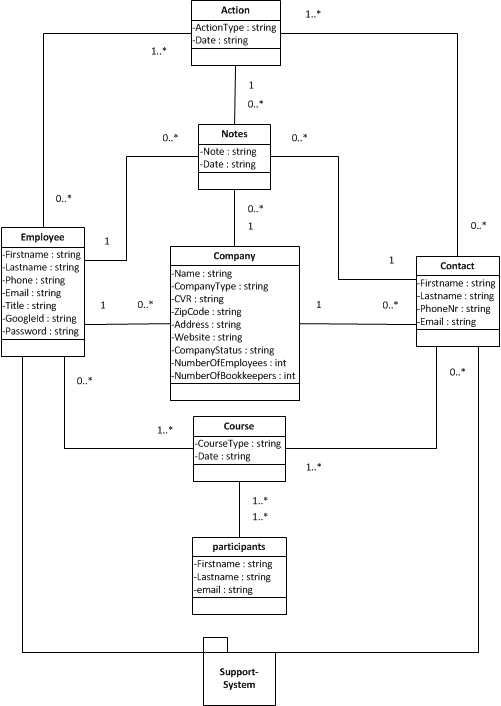
\includegraphics[width=0.75\textwidth]{domainModel}
	\caption{Dom�nemodel}
	
\end{figure}

Det kan ses p� modellen at en Employee ikke har direkte forbindelse til Contact, men i stedet har forbindelsen til Company. Dette er fordi de altid vil have alle firmaets kontakter. Action og Course er sat til Contact i stedet for Company for at en ansvarlig kontaktperson til netop den Action eller Kursus. Derudover er Participants sat ind for sig selv da det kan v�re ansatte i firmaet som man ellers ikke har nogen kontakt til.  Support-System er resten af det system der blev lavet under vores praktikophold. Modellen bag det har vi valgt at lave p� denne m�de for at holde de to projekter adskilt.
		
\subsection{Databasestruktur}
Database designet er lavet ud fra dom�ne modellen. Vi har fors�gt at holde tabellerne s� simple som muligt, det vil sige vi ikke blander data sammen. Derudover fors�ger vi at undg� null v�rdier samt redundans. Sidst vil vi normalisere databasen op til og med Boyce-Codd Normalform for at give os et bedre design, hvor vi minimerer redundans og opdaterer, inds�tter og sletter uregelm�ssigheder. 

Som det ses p� dom�ne modellen er der flere steder mange-til-mange relationer. For at styre dette i database sammenh�ng s�ttes en tabel ind imellem. Her vil de to fremmed n�gler til sammen lave en prim�r n�gle. Det kan blandt andet ses ved Employee og Action. Her vil der blive sat en ny tabel ind, som indeholder de to fremmed n�gler, som dens prim�re n�gle. 

De steder hvor der er 1-til-mange relationer vil der blive sat en fremmedn�gle p� den tabel der er mange af. Eksempelvis vil Company have mange kontakter, der s�ttes en fremmedn�gle p� kontakten s� den altid kan se hvilket firma den h�rer til. 
Hvis der havde v�ret 1-til-1 relationer v�lges en af tabellerne og vil fremmedn�glen ofte blive lagt p� den tabel med mindst v�rdier som peger p� den. Man vil ogs� fors�ge at ligge n�gler s�ledes man undg�r nulls.

1. NF kan blandt andet ses i vores Kontakt tabel hvor navnet p� kontakten er delt op i fornavn og efternavn, alts� atomare data.

2. NF kan ses flere steder i database da vi ikke har nogen attributter der er afh�ngig af dele af en n�gle.  

3. NF ses i det klassiske eksempel med post nummer og by. Da disse er afh�ngige af hinanden, og den prim�re n�gle flytter vi ud i en tabel for sig selv. 
\citep[p.348-361]{elmasri2007fundamentals}

\subsubsection{Beskrivelse af databasemodel}
Vi vil her beskrive sammenh�ngen mellem nogen af de tabeller hvor man ikke umiddelbart kan se hvad der menes.

\textbf{Company:} Denne tabel har flere tabeller knyttet til sig som kun indeholder en prim�r n�gle samt en enkelt attribut.(CompanyStatus, CycleState og CompanyTypes) Vi har lagt dem ud i tabeller for sig, fordi vi skal kunne s�ge og sortere p� dem. Det er lister med fastsatte v�rdier som kunden skal kunne v�lge ud fra.

\textbf{Titles:} Titles har to mange til mange tabeller, det er fordi en Employee kan have flere titler, samt mange titler kan have adgang til de samme steder i programmet. Det bruges til at styre hvor de forskellige Employees har adgang i programmet.

\textbf{Notes:} For at undg� at f� en masse null v�rdier har vi valgt at oprette en r�kke nye tabeller som ligner det man g�r ved mange til mange relationer. Her skal man dog v�re opm�rksom p� det faktisk kun er en, en til mange relation.  

\textbf{ValueList:} Kunden vil v�re i stand til at oprette dynamiske kolonner af bestemte typer. Derfor har vi lavet denne tabel som indeholder data samt en fremmed n�gle til infoList som fort�ller hvilken type data vi skal sorterer efter og hvad kolonnens navn er. Disse dynamiske kolonner er ens for alle Companies.

\chapter{Projektforl�b}
Her vil blive forklaret hvordan projektet er planlagt, og g� mere i detaljer omkring de enkelt sp�ndende omr�der i hvert sprint. Sprintet vil kort blive gennem�et hvorefter der vil blive kigget n�rmere p� nogle kodeeksempler.

I de fire sprints som forl�bet str�kker sig over, er hvert sprint delt op i 2 uger hvor af ca. 2� dag om ugen g�r med programmering mens de sidste uger af forl�bet g�r over i ren rapportskrivning. Denne struktur er valgt, for at f� skrevet lidt ned, mens det man har lavet stadig er nyt og friskt i hukommelsen. Ved ikke at lave for lange sprints f�r man oftere feedback p� produktet hvilket betyder, at man hurtigere kan rette til n�r eller hvis der kommer �ndringer.

\section{Product Backlog}
Product backloggen er en liste af alle de user stories der indg�r i projektet. Den er med til at give et godt overblik over hvad der mangler at blive lavet. Der kan l�bende blive tilf�jet nye user stories til product backloggen, som eventuelt kan blive taget med i det n�ste sprint. \ref{fig:Sprint 1 backlog}
\begin{figure}[H]
	\centering
		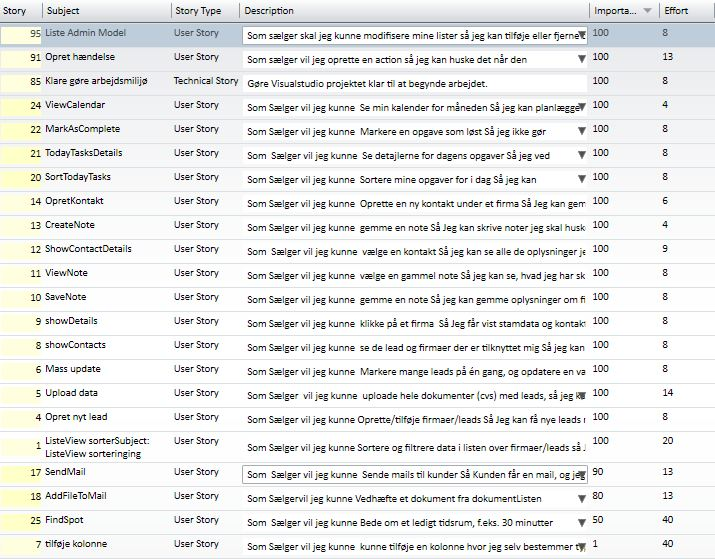
\includegraphics[width=1.00\textwidth]{Backlog.jpg}
	\caption{Backlog}
	\label{fig:Backlog}
\end{figure}

\section{Sprint 1}
I det f�rste sprint vil der altid g� tid med at f� sat arbejdsmilj� op, men da der skulle arbejdes videre p� et projekt som allerede havde sat op, var meget af dette allerede p� plads. Der skulle dog laves lidt, da der skulle omstruktureres p� opbygningen af projektet ved hj�lp af Areas i MVC 3. Derudover blev der ogs� en del refactoring af gamle klasser, fordi der blev lavet en hel del om i database designet, s� systemet kunne underst�tte al den nye funktionalitet.

\subsection{Sprint backlog}
Der blev ikke sat s� mange user stories ind i dette sprint for f� en god buffer til uventede problemer med arkitekturen og opstart af projektet. Der var ogs� lidt usikkerhed omkring hvor meget der kunne laves p� et sprint. 
Kolonnen "Effort" er det antal timer der er givet hver User Story. Der kan maximalt klares 53,2 i et sprint, og det viste sig at passe ret godt i f�rste sprint. 
\begin{figure}[H]
	\centering
		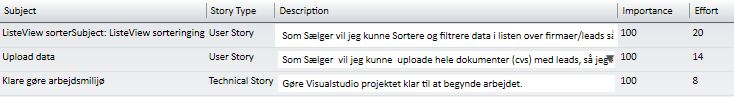
\includegraphics[width=1.00\textwidth]{Sprint1Backlog.jpg}
	\caption{Sprint 1 backlog}
	\label{fig:Sprint 1 backlog}
\end{figure}

\subsection{Burndown Chart}
Som burndown chartet viser, blev de f�rste opgaver l�st hurtigere end forventet, men det udlignede sig senere. Bufferen som bevidst var blevet sat ind i dette sprint for at f� en god start, blev der heldigvis ikke brug for. Det ses ogs� i form af, at alle opgaver var l�st en dag f�r sprintets deadline.
\begin{figure}[H]
	\centering
		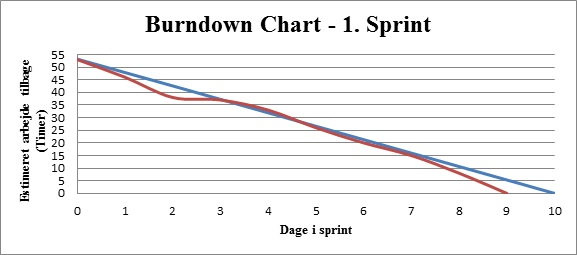
\includegraphics[width=1.00\textwidth]{Sprint1Burndown.jpg}
	\caption{Sprint 1 Burndown Chart}
	\label{fig:Sprint 1 Burndown Chart}
\end{figure}

\subsection{Udf�relse af Sprint 1}
Vi startede med at g�re arbejdsmilj�et klar til kunne h�ndtere den del af programmet der skulle h�ndtere salgsafdelingens omr�de. MVC 3 er heldigvis utrolig fleksibelt og vedligeholdsvenligt s� det gik nemt. Der opstod ikke nogen s�rlige problemer med hensyn til ops�ttelse af arbejdsmilj�et.

\subsubsection{User story - Upload data}
\textit{"`Som S�lger vil jeg kunne uploade hele dokumenter (cvs) med leads, s� jeg kan tilf�je mange kontakter p� �n gang. S� jeg hurtigt kan importere mange kontakter i stedet for at taste dem enkeltvis."'}

Som user story'et beskrive skal der kunne uploades en kommasepareret fil med leads, som efterf�lgende skal skrives ind i databasen. Her skal der selvf�lgelig tjekkes om der er dubletter s� der ikke uploades de samme leads flere gange. En dublet vil v�re et lead med samme CVR nummer. Skulle der v�re dubletter i filen vil man bliver ledt over p� en siden p� figur \ref{fig: csv-dubletter} hvor man vil se en liste med unikke leads og en liste med dubletter. Listen �verst er unikke leads, mens den nederste liste er dubletter fundet ud fra CVR-nummer. Her skal man s� v�lge den dublet man vil bruge, ved at afkrydse checkboxen ved siden af. Grunden til man skal kunne v�lge er at der sagtens kan v�re flere leads med samme CVR nummer i listerne, men med nyere stamdata. Det er s� op til s�lgeren at vurdere hvilke data er de nyeste.

\begin{figure}[H]
	\centering
		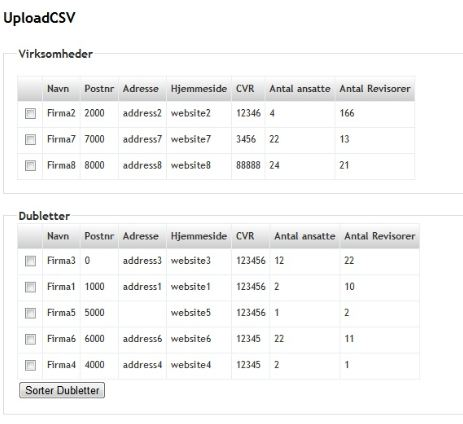
\includegraphics[width=.50\textwidth]{csv-dubletter.jpg}
	\caption{Liste af nye Leads og dubletter i csv-filen.}
	\label{fig: csv-dubletter}
\end{figure}

Undervejs i upload processen tjekkes der for dubletter i CSV filen, og dern�st i databasen inden der skrives hertil.

Det er kun den nederste liste man skal v�lge fra. Det er et af de steder vi gerne ville have haft tiden til at lave UI'et lidt om. Istedet for checkboxes skulle der v�re radiobuttons, da man kun skal kunne v�lge �t lead med samme CVR nummer, samt der selvf�lgelig ikke skal v�re nogen valgmulighed ved de unikke leads. Der var problmer med at f� grupperet radioknapperne ordenligt via razor. S� alternativet var at lave det om senere, og styre det via JavaScript og jQuery. Det n�ede vi desv�rre aldrig. 

Den �nskede CSV fil v�lges ved hj�lp af en simpel Web-form som man kan finde p� Leads-oversigts siden som vist p� figur \ref{fig: csv-form}. Det er vigtigt at et leads stamdata st�r i den rigtige r�kkef�lge fordi metoden ikke kan skelne mellem hvilke data det er den l�ser. Stamdata p� et lead vil v�re oplysnigner som CVR-nr, firmanavn, addresse, website osv.

\begin{figure}[H]
	\centering
		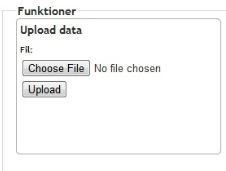
\includegraphics[width=0.70\textwidth]{csv-form.jpg}
	\caption{Webform til upload af CSV-fil}
	\label{fig: csv-form}
\end{figure}

Metoden i figur \ref{fig:csvupload} tjekker som det f�rste om filen overhovedet er blevet uploadet korrekt. S�fremt alt g�r godt, bliver filen kopieret over p� serveren, hvorefter stien til filen bliver sendt videre til metoden i figur \ref{fig: CSV-Reader} som er metoden der l�ser filen, mere om den senere.

\begin{figure}[H]
\lstset{language = CSharp}
\begin{lstlisting}
[HttpPost]
public ActionResult UploadCSV()
{
List<List<CSVCompanyWrap>> tempList = new List<List<CSVCompanyWrap>>();
            CSVList cvsList = new CSVList();
            try
            {
                HttpPostedFileBase file = Request.Files["uploadCSVContacts"];
                if (file != null && file.ContentLength > 0)
                {
                    string fileName = file.FileName;
                    string path = System.IO.Path.Combine(Server.MapPath("~/Uploads"), fileName);
                    file.SaveAs(path);

                    tempList = CSVReader(path);

                    cvsList.Companies = tempList[0];
                    cvsList.Doubles = tempList[1];
                }                
            }
            catch(Exception e)
            {...}            

            return View(cvsList);
        }
\end{lstlisting}
\caption{Metode til upload af CSV-fil i ContactListController.cs.}
\label{fig:csvupload}
\end{figure}

Da man kan sende objekter til vores UI med MVC 3, er der blevet lavet en wrapper klasse til at styre hvilke Company objekter der er blevet valgt p� UI'en via checkboxes. Se evt. Arkitektur afsnittet for uddybelse af Models og Views. 

CSVCompanyWrap er en wrapper-klasse til Company objekter da der skal v�re mulighed for at kunne v�lge hvilke leads der skal sorteres fra ved hj�lp af checkboxes. CSVCompanyWrap indeholder to simple Properties, en bool til at styre om checkboxen er markeret eller ej(true/false) og en property til det givne Company objekt. Ved at lave det p� denne m�de kan vi bruge MVC 3 til at sende en viewmodel til viewet p� figur \ref{fig: csv-dubletter}. N�r man s� laver en http-post sendes vores viewmodel tilbage til ContactListController hvor de forskellige checkboxe er valgt til og fra. 

CSVList er det vi kalder en ViewModel og indeholder to lister med CSVCompanyWrap objekter, dette er ogs� den model vores view i figur \ref{fig: csv-dubletter} forventer at modtage. De to lister svare til en r�kke leads og en r�kke dubletter. 
 
\begin{figure}[H]
\lstset{language = CSharp}
\begin{lstlisting}
private List<List<CSVCompanyWrap>> CSVReader(string filePath)
{
	List<List<CSVCompanyWrap>> fullList = new List<List<CSVCompanyWrap>>();
  List<CSVCompanyWrap> companies = new List<CSVCompanyWrap>();
  List<CSVCompanyWrap> dublets = new List<CSVCompanyWrap>();            
  try
  {
  	using (StreamReader reader = new StreamReader(filePath))
    {
    	string line;
      while ((line = reader.ReadLine()) != null)
      {
      	string[] lines = line.Split(';');
        short number;
        CSVCompanyWrap cw = new CSVCompanyWrap()
				{
        	Company = new Company()
          {
          	...       
          },
          Choosen = false
        };

        if (companies.Where(x => x.Company.Cvr.Equals(cw.Company.Cvr)).FirstOrDefault() != null)
        {
        	dublets.Add(cw);
          dublets.Add(companies.Where(x => x.Company.Cvr.Equals(cw.Company.Cvr)).Single());
          companies.Remove(companies.Where(x => x.Company.Cvr.Equals(cw.Company.Cvr)).Single());
        }
        else if (dublets.Where(c => c.Company.Cvr.Equals(cw.Company.Cvr)).FirstOrDefault() != null)
        {
        	dublets.Add(cw);
        }
        else
        {
        	companies.Add(cw);
      	}
    	}
  	}
  }
  catch (Exception e)
  {...}
  fullList.Add(companies);
	fullList.Add(dublets);
	return fullList;
}
\end{lstlisting}
\caption{Metode til l�sning af CSV-fil i ContactListController.cs.}
\label{fig: CSV-Reader}
\end{figure}

Metoden i figur \ref{fig: CSV-Reader} l�ser den uploadet CSV fil og splitter den op hver gang den st�der p� et ";". For hver linje i filen bliver der lavet et CSVCompanyWarp objekt, med et Company objekt, som stammer fra vores Entity framework, og en false bool.

Derefter tjekkes der s� om entity klassen Company eksistere i enten listen af dubletter eller companies. Findes den allerede bliver de flyttet til dubletter listen ellers bliver de lagt i companies listen. Det er ikke kun dubletten der bliver flyttet over i dubletter listen. Det g�r begge objekter da der senere skal v�lges hvilken der er rigtig, som forklaret tidligere er det op til s�lgeren at vurdere hvilket lead har de nyeste data.

Til sidst sendes de to lister tilbage til UploadCSV.cshtml som vist p� figur \ref{fig: csv-dubletter}. Her skal brugeren igen tage stilling til om hvilke data er de rigtige. Det er nemlig ikke n�dvendigvis det nyeste eller rigtige data som findes i CSV filen.

\begin{figure}[H]
\lstset{language = CSharp}
\begin{lstlisting}
[HttpPost]
public ActionResult SortDublets(CSVList csv)
{
    CSVList cvsList = new CSVList();

    foreach(var item in csv.Doubles)
    {
        if(item.Choosen)
        {
            item.Choosen = false;
            csv.Companies.Add(item);
        }
    }            
    cvsList.Companies = csv.Companies;

    return View("ConfirmCSV", cvsList);
}

\end{lstlisting}
\caption{Metode til sorting af dubletter i ContactListController.cs.}
\label{fig: Dublet-Sortering} 
\end{figure}

I figur \ref{fig: Dublet-Sortering} ses en simpel metode der flytter dubletter over i companies listen ud fra hvilken dublet-leads man valgte p� hjemmesiden. Herefter bliver man flytter over til ConfirmCSV.cshtml som ses i figur \ref{fig: godkendCSV}. Her skal man bekr�fte en sidste gang om man har valgt de rigtige leads.

\begin{figure}[H]
	\centering
		\includegraphics[width=.50\textwidth]{godkendcsv.jpg}
	\caption{Godkend stamdata af leads}
	\label{fig: godkendCSV}
\end{figure}

Det g�res som et simpelt tjek for at man ikke uploader noget data som ikke giver mening. Hvis man skulle v�lge et lead som man ikke vil have med pga. forkert data kan man v�lge den fra her. N�r det er gjort kan man upload sine data til databasen hvor der igen vil blive unders�gt om der er dubletter.  

\begin{figure}[H]
\lstset{language = CSharp}
\begin{lstlisting}
public ActionResult SubmitCSV(CSVList csv)
{
    List<CSVCompanyWrap> tempList = csv.Companies;            

    foreach(var item in tempList.ToList())
    {
        if (item.Choosen)
        {
            csv.Companies.Remove(item);
        }                
    }
    csv.Doubles = new LeadDetailsController(_db).LeadDetailsRepository.AddCompaniesFromCSV(csv);
    return View("ChooseDbDoubles", csv);
}

\end{lstlisting} 
\caption{Metode til at sortere valgte Leads i ContactListController.cs.}
\label{fig: Confirm-submit}
\end{figure}

Her l�ber metoden i figur \ref{fig: Confirm-submit} listen igennem for at se om brugeren skulle have fravalgt nogen leads, hvorefter de vil blive fjernet af listen. Til sidst sendes listen til repositoriet hvor de vil blive f�jet til databasen.

\begin{figure}[H]
\lstset{language = CSharp}
\begin{lstlisting}
public List<CSVCompanyWrap> AddCompaniesFromCSV(CSVList csv)
{
    List<CSVCompanyWrap> companyDoubles = new List<CSVCompanyWrap>();

    foreach(var item in csv.Companies.ToList())
    {
        CSVCompanyWrap comp = new CSVCompanyWrap()
        {
             Company = _db.Companies.Where(x => x.Cvr.Equals(item.Company.Cvr)).SingleOrDefault(),
                    Choosen = false
        };
                
        if (comp.Company != null)
        {
            companyDoubles.Add(item);
            companyDoubles.Add(comp);
        }
        else
        {                               
             _db.Companies.AddObject(item.Company);
             _db.SaveChanges();
        }
    }

    return companyDoubles;
}
\end{lstlisting}
\caption{Metode til at sortere dubletter i database.}
\label{fig: DB-dublets}
\end{figure}

Metoden i figur \ref{fig: DB-dublets} ligger i ContactRepository.cs. Derfor skrives og l�ses der direkte til databasen her. \_db er vores Entity Framework context.

Inden de endeligt bliver tilf�jet til databasen, unders�ges listen om der ogs� er dubletter i databasen. Det g�res ved at tr�kke et Company objekt ud fra database via CVR nummeret i den sorteret CSV liste. CVR-nummeret bruges fordi det er unikt og derfor ikke indeholder nulls eller ens v�rdier. SingleOrDefault() returnere enten et objekt eller null. Det vil sige, hvis metoden finder et objekt vil if-s�tning v�re true og s� vil de to dubletter blive skrevet i en liste som bliver sendt tilbage til brugeren. Hvis den ikke finder nogen objekter vil leadet fra CSV dokumentet bliver skrevet i databasen med det samme.

\begin{figure}[H]
	\centering
		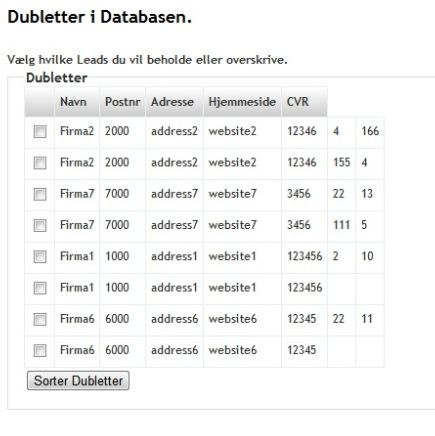
\includegraphics[width=.50\textwidth]{csvDBdubletter.jpg}
	\caption{Dubletter af sorteret CSV fil og Database}
	\label{fig: csv-db-dubletter}
\end{figure}

De dubletter der bliver fundet i CSV dokumentet og databasen skal sorteres p� samme m�de som tidligere af brugeren. Hvorefter de bliver sendt ned til repositoriet og overskriver objektet i databasen. Se figur \ref{fig: csv-db-dubletter}
 
\subsubsection{User Story - ListeView sortering}
\textit{"`Som S�lger vil jeg kunne Sortere og filtrere data i listen over firmaer/leads s� jeg kan f� leads frem i den r�kkef�lge jeg �nsker"'}

Et h�jt prioteret punkt p� listen over user stories, var muligheden for at sortere leads p� forskellige kriterier, s� man f.eks. kunne finde alle leads der skulle kontaktes inden for et bestemt datointerval, et bestemt postnummer eller virksomhedstype. Det skulle ogs� v�re muligt at filtrere p� flere kriterier p� en gang, s� man f.eks. kunne v�lge alle virksomheder inden for postnummer 8000-9000 med 20-100 medarbejdere. 
 
 Ideen er, at inde p� siden med leadsoversigten kan en bruger klikke p� en kolonneoverskrift, herefter vises en boks ud for musemark�ren, hvor brugeren kan s�tte filteret p� denne kolonne op. N�r brugeren uden for boksen, bliver filteret gemt og boksen skjules. Herefter kan brugeren enten s�tte flere filtre op, eller klikke p� "Filtr�r" hvorefter filtrene sendes til serveren, der returnerer de leads der falder inden for filtrenes parametre.
 
\textbf{Vise en Filterboks}\\
F�rste skridt var, at vise samtlige leads. Dette var en forholdsvis simpel opgave der var hurtigt l�st. N�ste step var, at lave mulighed for at tilf�je filtre. Det blev fastsl�et, at der grundl�ggende var tale om 4 typer filtre: tal, datoer, tekst og multiple-choice valg. Datatypen for kolonneoverskriften blev specificeret i et array, hvor der var et element for hver kolonne:
  
 I figur \ref{fig: headerDefinition} ses hvordan kolonneoverskrifterne og deres tilsvarende datatyper bindes sammen. Bem�rk l. 15-20, her hentes alle mulige employeeStatusser og alle employees ud af databasen. Resultatet af disse l�gges i de to arrays defineret i linjerne 8 og 9 - det er kolonner hvor der skal v�lges mellem flere fast definerede v�rdier.
 
  \begin{figure}[H]

\lstset{language = javascript}
 \begin{lstlisting}
filter = new Array();

categories = new Array();
categories["Navn"] = "tekst";
categories["Adresse"] = "tekst";
categories["By"] = "tekst";
categories["Postnummer"] = "number";
categories["Status"] = new Array();
categories["ES-kontakt"] = new Array();
categories["Sidste_Kontakt"] = "dato";
categories["Kontakt_igen"] = "dato";
categories["Web"] = "tekst";
categories["Ansatte"] = "number";

    var url = "getEmployeeStatus";
    $.getJSON(url, function (data) {
        categories["Status"] = data.states;
        categories["ES-kontakt"] = data.employees;
        
    });
 //$
 \end{lstlisting}
 \caption{Sammenbinding af overskrifter og typer}
  \label{fig: headerDefinition}
 \end{figure}
 
 Der blev lavet fire divs, som blev lagt som det sidste i body-delen af siden, med css-attributten \verb|display: none;| der betyder, at de ikke vises. Disse divs indeholder form-elementer der er er baseret p� de fire typer af data: dato, tekst, tal eller forudbestemte v�rdier som f.eks. status og ES-medarbejdere. 
 
 Disse 4 formularer ligger i bokse og repr�senterer hver af de fire typer af filtre. N�r brugeren klikker p� en kolonneoverskrift bliver der lavet en kopi af den relevante boks, s�fremt kassen ikke allerede eksisterer.
 
 \begin{figure}[H]
	\centering
		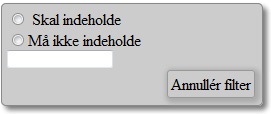
\includegraphics[width=.50\textwidth]{filterBoks.jpg}
	\caption{Eksempel p� filterboks - her til et tekst-filter}
	\label{fig:tekstFilterBoks}
\end{figure}
 
Koden i figur \ref{fig: clickHandler} h�ndterer klik p� en kolonneoverskrift, og visning af den boks, hvor brugeren bestemmer parametrene for filteret for denne kolonne. Hvis der allerede er sat et filter for denne kolonne vises den gamle filterboks, og hvis det er f�rste gang brugeren klikker p� netop denne kolonneoverskrift, oprettes der en ny filterboks som herefter vises.
 
 Der er i denne kodestump en del interessante punkter, det er v�rd at fremh�ve. F�rst og fremmest i linje 3 og 4, hvor chosenCategory ender med at indeholde hvilken slags datatype der er tale om. Herefter bestemmes det i l. 8-26 hvilken formulartype der skal vises. Id'et p� denne formular (som faktisk er en div) gemmes i variablen \verb|divToOpen|. I linje 26 skjules (ikke fjernes) evt. allerede viste filter-bokse. Efter, i linje 29 at have placeret filterboksen ved musemark�ren, bestemmes det om den valgte filterboks allerede eksisterer. 

Er det ikke tilf�ldet skal den valgte filterboks klones. Den nye boks bliver ikke tilf�jet dom-tr�et umiddelbart, men bliver lagt i variablen \verb|newElement|. Denne nye boks skal herefter have et id der dannes ud fra kolonneoverskriften og "\_filter", radio buttons skal have en name-attribut, s� de opf�rer sig korrekt, og kun h�rer sammen i d�n specifikke filterboks. Dette betyder, at radioknapper i f.eks. adresse-boksen ikke er k�det sammen med radioknapper i navne-boksen. I linje 36-41 bliver der for dato-felter initialiseret et jQuery plugin, s� der vises en dato-v�lger ved klik i disse bokse. Endelig appendes den nye boks til DOM-tr�et p� linje 46 og p� linje 48 vises den nye boks. 

Grunden til, at det bliver unders�gt om filterboksen allerede eksisterer, er for at man kan f� lov til at �ndre et allerede eksisterende filter.

Hvis den valgte boks allerede eksisterer i DOM-tr�et bliver det ganske enkelt lagt i newElement-variablen i l. 42. 

Som det sidste l�gges en overlay-div bag den nye filterboks, som, n�r der bliver klikket p� den, vil skjule filterboksen. Denne overlay-div eksisterer udelukkende med det form�l at registrere klik p� et hvilket som helst sted p� siden der ikke er filterboks.
 
 \begin{figure}[H]

 \lstset{language = javascript}
 
 \begin{lstlisting}
 /// Klik p� en kolonneoverskrift
$('#contactTable th').click(function (e) {
    var chosenField = $(this).text().replace(" ", "_");
    var chosenCategory = categories[chosenField];

    var divToOpen;

    if ($.isArray(chosenCategory)) {

        divToOpen = "selectFilter";
        $('#selectedVal').html('');
        $.each(chosenCategory, function () {
            var value = $(this)[0].value;
            var text = $(this)[0].text;
            $('#selectedVal').append('<option value="' + value + '">' + text + '</option>');
        });
    }
    else if (chosenCategory == "dato") {
        divToOpen = "dateFilter";
    }
    else if (chosenCategory == "number") {
        divToOpen = "numberFilter";
    }
    else if (chosenCategory == "tekst") {
        divToOpen = "textFilter";
    }

    $('.filterDiv').hide();
    $("#" + divToOpen).css('top', e.pageY + 7).css('left', e.pageX + 7);
    var suffix = "_Filter";

    if ($('#' + chosenField + suffix).length == 0) {
        newElement = $('#' + divToOpen).clone();
        newElement.attr('id', chosenField + suffix);
        newElement.children('input[type="radio"]').attr('name', chosenField + 'RadioBtn');
        $(newElement).find('.datePickerField').datepicker({
            showWeek: true,
            firstDay: 1,
            showOtherMonths: true,
            selectOtherMonths: true
        });
        $('body').append(newElement);
				//$('body').after(newElement);
    }
    else {
        newElement = $('#' + chosenField + suffix);
    }
    $(newElement).fadeIn("fast");
    $(newElement).after("<div class='darkClass'></div>");
});


\end{lstlisting}
\caption{Komplet eventhandler for klik p� kolonneoverskrift}
 \label{fig: clickHandler}
\end{figure}

\textbf{Gemme filter}\\
N�r brugeren klikker udenfor filterboksen (dvs. p� overlay-div'en) bliver filteret gemt. Det f�rste der sker, er at overlay-div'en fjernes, herefter bliver div'en med filterboksen lagt i en variabel og gemt, s� brugeren ikke kan se den l�ngere. Det n�ste der sker, er at filterets kategori bliver bestemt ud fra id p� filterboksen og ud fra denne kategori, filterets type (tekst, tal, dato eller multiple choice). Baseret p� typen bliver filteret nu behandlet, s� det kan gemmes i et array "filters", der best�r af en r�kke filter-objekter. Til sidst bliver den relevante kolonneoverskrift markeret med en streg under teksten, s� man kan se, at der er oprettet et filter for denne kategori.

I figur \ref{fig: hideFilterDiv} ses hvordan overlay-div'en fjernes, filterdiven skjules og id'en hentes ud (l. 2-6). I linjerne 14-20 ses et eksempel p�, at der gemmes en tekst-v�rdi. I filter-objektet gemmes egenskaberne values, criteria, type og category. Values indeholder v�rdien/erne. Ved datoer og tal er values altid et array, da der skal v�re mulighed for en �vre og nedre gr�nsev�rdi. Criteria indeholder kriteriet for filteret (st�rre end, mindre end, m� indeholde, m� ikke indeholde osv). Type er ganske enkelt type af filteret og category indeholder kategorien.
 \begin{figure}[H]

 \lstset{language = javascript}
 
 \begin{lstlisting}
 $('body').delegate('.darkClass', 'click', function () {
    $('.darkClass').remove();

    var newlyHiddenElement = $('.filterDiv:visible');
    newlyHiddenElement.hide();
    var hiddenElementId = newlyHiddenElement.attr('id').split("_");

    if (hiddenElementId.length == 3)
        category = hiddenElementId[0] + "_" + hiddenElementId[1];
    else
        category = hiddenElementId[0];
    var categoryType = categories[category];
    switch (categoryType) {
        case "tekst":

            var criteria = parseInt($(newlyHiddenElement).children('input:radio:checked').val());
            var value = new Array($(newlyHiddenElement).children('input[type="text"]').val());
            if (value != "")
                filter[category] = { values: value, criteria: criteria, type: "text", category: category };
            break;
            //$
            ...
                
\end{lstlisting}
\caption{Uddrag af eventhandler for oprettelse af filter}
 \label{fig: hideFilterDiv}
\end{figure}


\textbf{Anvend filter}\\
N�r bugeren klikker p� "Filtr�r" blive der oprettet et asynkront kald, der indeholder filter-betingelserne (fig \ref{fig: sendFilter}, l. 2-9). Dette kald sendes til serveren, der filtrerer. N�r klienten modtager resultatet fjernes f�rst den gamle oversigt over leads (l. 11), hvorefter listen med resultater l�bes igennem. I kodeeksemplet er det i linje 13, at l�kken starter. Dato-felter bliver formatteret til et fornuftigt format (udeladt), herefter samles en ny r�kke (l. 19-26 - dele udeladt). Som det sidste tilf�jes den netop oprettede r�kke til DOM-tr�et (l. 27)

 Serverside-delen af filtreringen bliver n�rmere forklare p� s. \pageref{chap: decorator} under overskriften "Implementering".


 \begin{figure}[H]

 \lstset{language = javascript}
 
 \begin{lstlisting}
formattedFilter = JSON.stringify(newFilter);
$.ajax({
    url: "ApplyFilter",
    data: formattedFilter,
    type: "POST",
    dataType: "json",
    contentType: 'application/json; charset= utf-8',
    processData: false,
    success: function (data) {

        $('#contactTable tr:nth-child(n+2)').remove();

        for (var company in data.returnCompanies) {
            var currentCompany = (data.returnCompanies[company]);
            //console.log(currentCompany);
       
       			...

            var newTr = "<tr>";
            newTr += '<td><input id="check_' + currentCompany.Id + '" type="checkbox" value="' + currentCompany.Id + '"></td>';
            newTr += '<td><p>' + currentCompany.Navn + '</p></td>';
						
						...
						
            newTr += '<td><p>' + currentCompany.Ansatte + '</p></td>';
            newTr += "</tr>";
            $('#contactTable tbody').append(newTr);
        }
    }
});
//$
 \end{lstlisting}
\caption{Uddrag af selve filtreringen, clientside}
 \label{fig: sendFilter}
\end{figure}

Det er et bevidst valg, at filtrene ikke bliver anvendt i samme �jeblik filteret bliver oprettet. Dette skyldes, at der skal v�re tid til at oprette flere filtre af gangen, uden at skulle vente p�, at resultatet af den forrige filtrering bliver loadet og vist.

\subsection{Retrospective}
Det f�rste sprint gik utroligt godt, vi fik overraskende f� problemer med at klarg�re milj�et, hvor vi ellers havde regnet med der kunne opst� flere problemer. Vi fik set en af MVC's st�rke sider, ved at man nemt kan vedligeholde det, og tilf�je store �ndringer til det. Samtidig fik vi ogs� set hvor nemt det bliver at lave selv forholdsvis store �ndringer i databasen n�r man bruger entity frameworket. Der blev selvf�lgelig en del refactoring i vores gamle projekt, men p� trods af de store �ndringer var det hurtigt og nemt at f� til at virke igen. Blandt andet skulle vi implementere repository pattern, udover at f� adskilt vores database kald fra controllerne fik vi ogs� bedre mulighed for at unit teste. Derudover var der en del �ndringer i databasen omkring vores Customer og Company klasser, men da Enity frameworket laver vores modellag var det ogs� forholdsvist nemt at skrive om. 

Da vores support del af programmet l� i roden af vores MVC3 projekt skulle der ogs� laves en anden mappe struktur her. Det viste sig at v�re nemt at g�re med MVCs Areas som bet�d vi mere eller mindre bare kunne flytte hele projektet ind i en ny mappe, og samtidig bevare al funktionalitet, og mens alle links inden for det Area stadig pegede det rigtige sted hen.

Refactoring blev en n�dvendighed da systemet skulle udvides, men ogs� som en del af at forbedre og optimere den kode som allerede var skrevet. Da der bruges mange nye teknologier finder man ofte nye, smartere og mere rigtige m�der at g�r tingene p� i forhold til de framework man bruger. 
 

\section{Sprint 2}
I sprint 2 var der mange sm� opgaver. Det var mange CRUD opgaver, hvor der blev brugt en hel del JavaScript p� at f� lavet en GUI uden for mange synkrone serverkald. Det er ogs� derfor noget s� simpelt som at vise nogle detaljer tager s� "lang" tid som det gjorde her. Det meste af GUI'en kom p� plads i dette sprint.

\subsection{Sprint Backlog}
Efter sprint 1 blev vores sprint "Capacity" bekr�ftet, derfor vi var mere rolige ved at s�tte mange user stories i dette sprint og udlade den buffer vi havde sidst. Det er en masse sm� Stories som samtidig kr�ver at der blev lavet en del GUI. 
\begin{figure}[H]
	\centering
		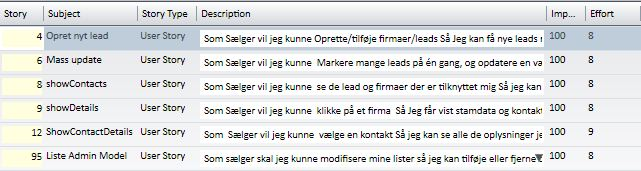
\includegraphics[width=1.00\textwidth]{Sprint2Backlog.jpg}
	\caption{Sprint 2 backlog}
	\label{fig:Sprint 2 backlog}
\end{figure}

\subsection{Burndown Chart}
Vi kom lidt bagud til at starte med, det var hovedsageligt mass-update der tog lidt l�ngere tid end forventet. Da mange af opgaverne mindede om hinanden, indhentede vi den tabte tid igen og n�ede i m�l til tiden.
\begin{figure}[H]
	\centering
		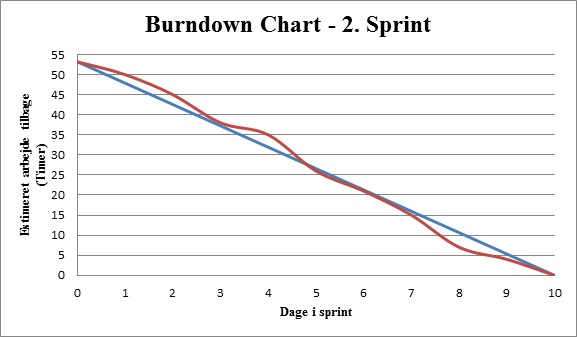
\includegraphics[width=1.00\textwidth]{Sprint2Burndown.jpg}
	\caption{Sprint 2 Burndown Chart}
	\label{fig:Sprint 2 Burndown Chart}
\end{figure}

\subsection{Udf�relse af sprint 2}
\subsubsection{User story - Mass update}
\textit{"`Som s�lger vil jeg kunne Markere mange leads p� �n gang, og opdatere en variabel der g�lder for dem alle"'}

F�rste punkt, var at implementere en m�de, s� brugeren kunne v�lge hvilke leads der skal opdateres. Dette var forholdsvist simpelt, da der ganske enkelt blev tilf�jet en checkbox yderst til venstre, der havde companyId som value. N�ste del var at lave en m�de, hvor brugeren kunne fort�lle hvilken kategori der skulle opdateres, og hvad den nye v�rdi skulle v�re. Der blev tilf�jet et element i den �verste bar, hvor man kunne v�lge kategori, denne select-liste blev lavet ud fra hvilke kategorier der fandtes i tabellen, som set i fig \ref{fig:tabelLoop}

Denne funktion findes p� listen over leads, og skal bruges til at opdatere data for mange leads p� �n gang. F.eks. hvis mange firmaer f�r ny kontaktperson ved ES.

F�rste punkt, var at implementere en m�de, s� brugeren kunne v�lge hvilke leads der skal opdateres. Dette var forholdsvist simpelt, da der ganske enkelt blev tilf�jet en checkbox yderst til venstre, der havde companyId som value. N�ste del var, at lave en m�de, hvor brugeren kunne fort�lle hvilken kategori der skulle opdateres, og hvad den nye v�rdi skulle v�re. Der blev tilf�jet et element i den �verste bar, hvor man kunne v�lge kategori, denne select-liste blev lavet ud fra hvilke kategorier der fandtes i tabellen, som set i fig \ref{fig:tabelLoop}
\begin{figure}[H]
\lstset{language = javascript}
\begin{lstlisting}
$.each($('#contactTable th:nth-child(n+2)'), function () {
    $('#categoryToUpdate').append('<option value="' + i + '">' + $(this).text() + '</option>');
    i++;
});
\end{lstlisting}
\caption{L�kke der fylder selectboxen baseret p� kolonner i tabellen}
\label{fig:tabelLoop}
\end{figure}
\textbf{Valg af kategori}

I figur \ref{fig:massUpdateEventhandler} ses eventhandleren der h�ndterer valg af kategori der skal opdateres. N�r brugeren v�lger kategorien, bliver typen bestemt p� samme m�de som ved oprettelse af et filter (l. 2-3) . Hvis der er tale om et array, bliver der lavet en selectbox med de foruddefinerede v�rdier (l. 5-14), og ellers bliver der oprettet et inputfelt. Hvis der er tale om et datofelt bliver dato-plugin'en ogs� initialiseret (l. 15-23).
\begin{figure}[H]
\lstset{language = javascript}
\begin{lstlisting}
$('body').delegate('#categoryToUpdate option', 'click', function () {
	var chosenField = $(this).text().replace(" ", "_");
  var chosenCategory = categories[chosenField];

  if ($.isArray(chosenCategory)) {
  	$('#massUpdateInput').html('<select id="updateInput"></select>');
    $.each(chosenCategory, function () {
    	var value = $(this)[0].value;
      var text = $(this)[0].text;

      $('#updateInput').append('<option value="' + value + '">' + text + '</option>');

		});
	}
  else if (chosenCategory == "dato") {
	  $('#massUpdateInput').html('<input type="text" id="updateInput" class="datePickerField" />');
	  $('#updateInput').datepicker({
		  showWeek: true,
		  firstDay: 1,
		  showOtherMonths: true,
		  selectOtherMonths: true
	  });
	}
  else if (chosenCategory == "number") {
      $('#massUpdateInput').html('<input type="text" id="updateInput" value="nummerfelt" />');
  }
  else if (chosenCategory == "tekst") {
      $('#massUpdateInput').html('<input type="text" id="updateInput" value="tekst" />');
  }
});
    
	\end{lstlisting}
  \caption{Eventhandleren for valg af kategori}
  \label{fig:massUpdateEventhandler}
\end{figure}

\textbf{Gemme v�rdier}
N�r v�rdierne skal gemmes, skal siden finde ud af, hvilket firma-id der er sat hak ved i oversigten, og hvad den nye v�rdi er. At finde virksomhederne er forholdsvist simpelt, der laves en jQuery-l�kke der l�ber igennem samtlige checkboxe inde i td-tags, der er checked. Herefter er det bare at tage value af disse checkboxes og tilf�je dem til et array over companyId's.
N�r virksomhederne er kendte, skal den nye v�rdi tr�kkes ud. Disse v�rdier skal l�gges i to variabler, newVal og newText. Hvis der er tale om tal, datoer eller tekst, er disse to identiske. Hvis der derimod er tale om data fra en selectbox, er der forskel p� disse to. Variablen newVal er v�rdien (value) fra selectboxen, mens newText indeholder teksten. 

N�r v�rdierne er hentet ud, er der kun tilbage at sende foresp�rgslen til serveren, som vil opdatere v�rdierne, skrive de nye v�rdier i tabellen og afmarkere alle selectboxe.


\subsubsection{ShowDetails}
\textit{"`Som s�lger vil jeg kunne klikke p� et firma, s� jeg f�r vist stamdata og kontakter"'}

Denne userstory h�nger t�t sammen med den n�ste - at se detajler for kontakter. Begge userstories realiseres p� contactDetail-siden.

F�rst skulle oversigten over virksomheder vises, denne oversigt blev lavet som et partial view, der blev vist. Controlleren for dette view tager en enkelt parameter, der afg�rer hvordan virksomhederne sorteres. Sorteringsr�kkef�lgen �ndres ved klik i kolonneoversigten.

\begin{figure}[H]
\lstset{language = CSharp}
\begin{lstlisting}
public ActionResult _LeadsList(string SortOrder)
{
    List<CompanyList> companies = new List<CompanyList>();
    companies = repo.GetCompaniesList(companies, SortOrder);

    return PartialView("_LeadsList", companies);
}
\end{lstlisting}
\caption{Controller for Oversigt over virksomheder}
\label{fig:companyOverViewController}
\end{figure}
Herefter skulle klik p� en virksomhed p� listen h�ndteres. Det blev vurderet, at det bedste ville v�re, at hente virksomheden via et asynkront kald, der hentede s� meget som muligt ind p� �n gang. Derfor hentes stamdata for virksomheden ind som partial view. Dette partial view returnerer en m�ndge html, som s�ttes ind p� siden via jQuery. Samtidig foretages der et andet asynkront kald, der henter alle virksomhedens kontakter. Disse kontakter og deres tilh�rende data gemmes i en variabal, da de bekvemt nok kommer tilbage, pakket p�nt ind i et array. I figur \ref{fig:getContacts} ses hvordan listen samles p� serveren og herefter returneres som et JSON-objekt.

\begin{figure}[H]
\lstset{language = CSharp}
\begin{lstlisting}
public ActionResult getContacts(int companyId)
{
	var contacts = repo.GetContactsByCompany(companyId);
	string navn = repo.GetCompany(companyId).Name;
	var contactList = (
		from c in contacts
		select new
		{
		   firstName = c.Firstname,
		   lastName = c.Lastname,
		   contactId = c.Contactsid,
		   phone = c.Phone,
		   cell = c.Mobilephone,
		   actions = (from b in c.Actions
		              orderby b.Date descending
		              where b.Date < DateTime.Now
		              select new
		              {
		                  actionId = b.Actionsid,
		                  date = b.Date,
		                  desc = b.Description,
		                  type = b.Actiontype.Actiontypesid,
		                  employees = (from d in b.Employees
		                               select 
		                                   d.Firstname + " "+ d.Lastname)
		                }),
		   email = c.Email,
	...
	return Json(new { contactList, navn, notes }, JsonRequestBehavior.AllowGet);
}

\end{lstlisting}
\caption{Listen over kontakter s�ttes sammen.}
\label{fig:getContacts}
\end{figure}Ud fra dette objekt laves oversigten over kontakter i h�jre side. Ved at hente al information ud p� �n gang spares tid n�r brugeren klikker p� en kontakt. Vi vurderede, at den ekstra tid for det ekstra kald, ikke ville betyder noget, i forhold til ventetiden ved at lave et ekstra seperat kald ved klik p� oversigten. Hvis det senere viser sig, at det er meget store m�ndger data der skal hentes, som vil for�rsage en v�sentlig ventetid, kan det let lade sig g�re, at data om en enkelt kontakt f�rst hentes ud ved klik p� den specifikke kontakt.
\subsubsection{ShowContactDetails}
\textit{"`Som s�lger vil jeg kunne v�lge en kontakt, s� jeg kan se alle oplysninger jeg har gemt om kontakten"'}

N�r en bruger klikker p� en kontakt i oversigten, udledes kontaktens id af id'et p� den div, der blev klikket p�, hvorefter der s�tte to cookies, �n med contactId'et, og en med nummeret p� den kontakt-div der blev klikket p�:

\begin{figure}[H]
\lstset{language = javascript}
\begin{lstlisting}

$('body').delegate('.contactDiv', 'click', function ()
{

	clickedElement = $(this).attr('id').split("_")[1];
	var clickedContact = contactList[clickedElement];
	setCookie("actualContactId", clickedContact.contactId);
	setCookie("contactId", clickedElement);
		\end{lstlisting}
  \caption{Hentning af data om den valgte kontakt.}
  \label{fig:clickedContactHandlerFirst}
\end{figure}

Herefter fyldes data i de felter hvor de h�rer til. Siden er i forvejen opbygget med en r�kke div's der har et span-element som child. Dette span-element indeholder de forskellige data og bruges ogs� til at redigere data. Da variablen clickedContact indeholder alle oplysninger om kontakten er det en forholdsvist simpel ting at udfylde felterne.
	\begin{figure}[H]
\lstset{language = javascript}
\begin{lstlisting}
	var esContact = clickedContact.ESContact;
	$('#chosenContact').val(clickedContact.contactId);
	$('#navn_contact_div').children('span').text(clickedContact.firstName + " " + clickedContact.lastName);
	$('#mail_contact_div').children('span').text(clickedContact.email);
	$('#telefon_contact_div').children('span').text(clickedContact.phone);
	$('#cell_contact_div').children('span').text(clickedContact.cell);
	$('#medarb_contact_div').children('span').text(esContact.firstName + " " + esContact.lastName);
\end{lstlisting}
\caption{Visning af basal data for kontakt}
\label{fig:contactDetailsShowingBasicData}
\end{figure}

Det n�ste der sker, er at actions skal vises. Igen ligger alle actions allerede i  clickedContact-objektet. Af hensyn til overblikket skal der h�jst vises de tre sidste actions, l�ngere nede p� siden findes en komplet oversigt over alle actions p� den aktuelle kontakt. Igen er der allerede en div med et span-element som child, der er klar til at holde informationen:
\begin{figure}[H]
\lstset{language = javascript}
\begin{lstlisting}
var prevActions = ""

maxActions = (clickedContact.actions.length > 3) ? 3 : clickedContact.actions.length;

for (var actionNo = 0; actionNo < maxActions; actionNo++)
{
	var action = clickedContact.actions[actionNo];
	var newDate = parseInt(action.date.replace(/[^\d.]/g, ""));

	prevActions += " (" + getDateYear(newDate) + ") " + action.desc + "<br />";
}

$('#lastContact_contact_div').children('span').html('');
$('#lastContact_contact_div').children('span').html(prevActions);
	\end{lstlisting}
	\caption{Tilf�jelse af actions i oversigten}
	\label{fig:contactDetailsShowActions}
\end{figure}
	
	
	\begin{figure}[H]
\lstset{language = javascript}
\begin{lstlisting}
$('.companyNote').remove();

//Viser notes for kontakten
for (var noteId in clickedContact.notes)
{
	var note = clickedContact.notes[noteId];

	var entryDate = eval("new " + (note.date).replace(/\//gi, ""));
	note.dato = (dateFormat(entryDate)).replace(/\//gi, "-");

	$('#contactNotes').after("<div class='companyAction'><div class='companyNote' id='compNote_" + note.notesId + "'><span  class='companyNoteHeader'>" + note.employee + " - " + note.dato + "</span><div class='noteContent'>" + note.content + "</div></div></div>");
}
	\end{lstlisting}
	\caption{Visning af notes for den valgte kontakt}
	\label{fig:contactDetailsShowNotes}
\end{figure}
Som det sidste skal der vises opkald og m�der med kontakten, hvilket ogs� er forholdsvist simpelt.
		\begin{figure}[H]
\lstset{language = javascript}
\begin{lstlisting}
	//Viser opkald for kontakten
	for (var actionId in clickedContact.actions)
	{
		var action = clickedContact.actions[actionId];
		var entryDate = eval("new " + (action.date).replace(/\//gi, ""));
		action.dato = (dateFormat(entryDate)).replace(/\//gi, "-");
		var element = "";
		if (action.type == 1)
			element = "opkald";
		if (action.type == 2)
			element = "meetings";

		if (element != "")
			$('#' + element).after("<div class='companyAction'><div class='companyNote' id='compNote_" + action.actionId + "'><span  class='companyNoteHeader'>" + action.dato + "</span><div class='noteContent'>" + action.desc + "</div></div></div>");

	}
});

//$
	\end{lstlisting}
  \caption{Eventhandleren for valg af kategori}
  \label{fig:clickedContactHandler}
\end{figure}

I disse to user stories blev der lagt en del tanker bag opbygningen af den del, hvor stamdata som telefonnummer, adresse, navn osv. blev vist - b�de for firma og kontakt. Grunden var, at det skulle v�re nemt at �ndre oplysninger. Product owner �nskede, at det skulle v�re s� simpelt s� muligt. Det blev vurderet, at det nemmeste ville v�re en l�sning, hvor brugeren klikkede p� en information som f.eks. telefonnummeret, hvorefter teksten �ndredes til et tekst-felt. Efter man har �ndret oplysningen og klikker udenfor tekstfeltet, �ndres det tilbage til tekst og databasen opdateres.

Dette resulterede i en opbygning, hvor hver information havde f�lgende html:
\begin{figure}[H]
\lstset{language = html}
\begin{lstlisting}
<div id="city_firm_div" class="infoDiv">
	<span>@Model.City.Cityname</span></div>
</div>  
\end{lstlisting}
\caption{Eksempel p� datavisning.}
\label{fig:showDataDetail}
\end{figure}
Med denne opbygning var det nemt at lave en jQuery eventhandler der reagerede p� klik i span i divs med klassen "infoDiv". Teksten i span'en kunne ogs� nemt udskiftes med en infoboks. Denne infoboks har s� en eventhandler p�, der reagerede n�r tekstboksen mistede fokus. Via $delegate$-funktionen var det ikke n�dvendigt at l�gge eventhandleren p� hver gang.

Desuden var det ogs� simpelt, for information omkring den enkelte kontakt, at udfylde felterne, da det var span'en i den relevante div der skulle udfyldes via jquery's $.html()$-funktion. Denne funktion giver mulighed for at inds�tte html i et bestemt element.
\subsection{Retrospective}
Det var et forholdsvis nemt sprint uden de helt store udfordringer, men ogs� et vigtigt sprint da der kom en masse GUI p� plads. Det var rart at have noget rigtigt at vise vores product owner. 

Vi snakkede ogs� om at vi skal passe p� med ikke at k�le for meget ved de helt sm� detaljer. Derudover skal vi holde os til de user stories/tasks der er skrevet ned og ikke begynde at lave ny funktionalitet, ogs� kaldet "Feature Creep". P� trods af det var det et godt sprint der endnu gang endte til tiden, men igen ogs� et sprint uden de store udfordringer. 

\section{Sprint 3}
I sprint 3 tog vi hul p� Note delen af vores system, samt det at kunne oprette en h�ndelse, hvor den sidst n�vnte nok er det mest interessante i dette sprint. Notes delen var en nogenlunde simpel CRUD operation, mens h�ndelse var noget mere vanskelig da der skulle synkroniseres med Googles kalender. 

Derudover skulle der ogs� laves s� man kunne se sin kalender samt oprettelse af Kontakter.

\subsection{Sprint Backlog}
Der var forholdsvis mange stories i dette sprint, hvor "Opret h�ndelse" var den klart mest komplekse som kunne skabe lidt problemer hvis vi var uheldige. Der var ogs� en del research involveret med den da vi skulle synkronisere den med Googles Calendar.

\begin{figure}[H]
	\centering
		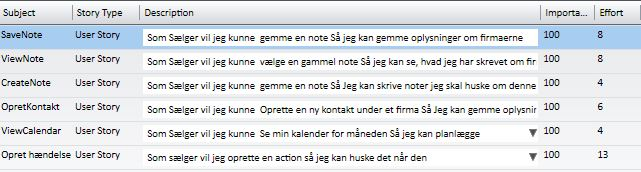
\includegraphics[width=1.00\textwidth]{Sprint3Backlog.jpg}
	\caption{Sprint 3 backlog}
	\label{fig:Sprint 3 backlog}
\end{figure}

\subsection{Burndown Chart}
Som det kan ses p� burndown chartet gik det helt galt i dette sprint. Ikke s� meget fordi vores estimater ikke holdte, men fordi firmaet vi skrev opgave hos gik konkurs. Det fik selvf�lgelig den betydning at vores udviklingsmilj� blev lagt ned og gjorde det umuligt at forts�tte, da vi brugte deres servere. De ville heldigvis gerne hj�lpe os f�rdige med projektet s� serveren blev sat op igen p� en ny adresse hvor vi s� kunne udvikle videre hjemmefra. Det bet�d dog der var et par dage mens serverne blev flyttet som ogs� kan ses efter dag 1. Da serverne kommer igen forts�tter vi arbejdet og n�r n�sten igennem sprintet p� trods af det store slag det var at firmaet gik ned. Da det var en private bredb�nds linje serverne blev stillet op p�, bet�d det desv�rre at forbindelsen var en smule ustabil hvilket kan ses p� dag 6.

Det var prim�rt "Opret h�ndelse" vi ikke n�ede at blive f�rdig med.

\begin{figure}[H]
	\centering
		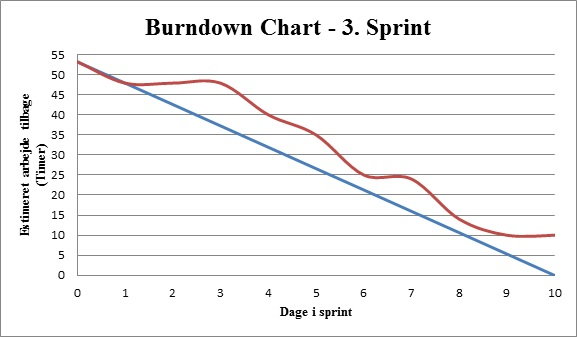
\includegraphics[width=1.00\textwidth]{Sprint3Burndown.jpg}
	\caption{Sprint 3 Burndown Chart}
	\label{fig:Sprint 3 Burndown Chart}
\end{figure}

\subsection{Udf�relse af sprint 3}
Hvis man ser bort fra problemerne omkring serverne, gik sprintet s�dan set udm�rket, hvor vi n�ede de fleste af vores user stories. Visning og oprettelse af Notes blev lavet som de f�rste, sammen med oprettelse af Kontakt. 

View Calendar havde vi lavet en proof of concept p�, s� den burde v�re nem at implementere ordenligt i systemet. Derudover manglede opret h�ndelse at blive lavet f�rdig, det lykkedes os dog at lave en stor del af den.

\subsubsection{User Story - Opret H�ndelse}
\textit{"Som s�lger vil jeg oprette en action s� jeg kan huske det n�r den ogs� blive skrevet til min google-kalender"}

Det vores product-owner egentlig �nskede var t�t p� en kopi af Googles egen m�de at g�re det p�. Det bet�d at udover de mest basale features som overskrift, beskrivelse, til og fra tidspunkter, skulle der ogs� laves gentagelser. Det vil sige der skulle v�re mulighed for at gentage en h�ndelse X antal gange hver tirsdag, for eksempel. 

Det valgte vi at l�se ved at lave en tabel til kun at styre gentagelser, samt en til at styre datoerne.

\begin{figure}[H]
	\centering
		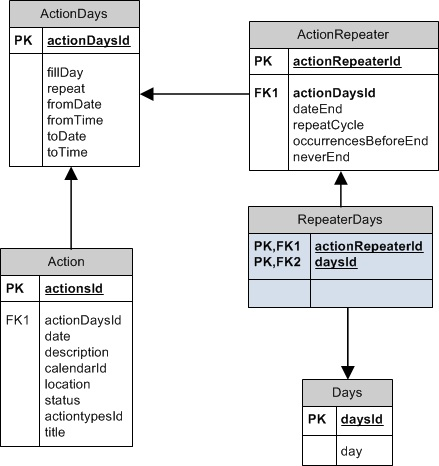
\includegraphics[width=1.00\textwidth]{actiondb.jpg}
	\caption{Udsnit af databasediagram.}
	\label{fig: Actiondb}
\end{figure}

Som det kan ses p� figur \ref {fig: Actiondb} er der ogs� en date p� Action. Dette er noget vi selvf�lgelig vil refactor om, s� vi ikke har det samme data to steder. Men grundet vores tidsm�ssige problemer i dette sprint, n�ede vi det aldrig, men vi er dog opm�rksomme p� dette. 

Da oprettelse af en h�ndelse er en del af et st�rre View med mange Models bruger man et PartialView. Det vil sige man kan s�tte et View ind i et View og p� den m�de dele sine UI op i de forskellige sektioner man nu har p� en side. Man kan ogs� sende en anden Model til sit partialView, det g�r det utrolig nemt og smart at bygge sine sider op p� den m�de.

\begin{figure}[H]
\lstset{language = CSharp}
\begin{lstlisting}
<div id="detaljer" class="mainWindow">
   ...
        <fieldset>
            <legend>H�ndelser</legend>        
            
            @using (Html.BeginForm())
            {                
                @Html.Action("Action")            
            }
        </fieldset>
...
</div>
\end{lstlisting} 
\caption{Importerer et PartialView.}
\label{fig: PartialView}
\end{figure}

P� figur \ref{fig: PartialView} ses det View der kalder det partialView som indeholder den kode der skal til for at vise vores H�ndelses sektion. Der kan blandt andet bruges en "helper" kaldet Action. Som parameter tager den her navnet p� den metode som skal kaldes i controlleren. At helperen og metoden der bliver kaldt, begge hedder Action er tilf�ldigt.

\begin{figure}[H]
\lstset{language = CSharp}
\begin{lstlisting}
[ChildActionOnly]
public ActionResult Action()
{
    ActionViewModel avm = new ActionViewModel();
    avm.ActionType = repo.GetActionTypes();

    return PartialView("ActionViewModel", avm);
}
\end{lstlisting} 
\caption{ChildActionOnly Metode}
\label{fig: ChildActionOnly}
\end{figure}

P� figur \ref{fig: ChildActionOnly} ses den metode som blev kaldt fra vores View i figur \ref{fig: PartialView}. Attributten [ChildActionOnly] g�r at der kun kan kaldes fra et View. Selve metoden henter en liste af ActionTyper som bliver lagt i vores partialviews model. Listen bruges til at fylde en dropdownbox med data. Til sidst returnerer vi et PartialView(), som her tager to parameter. Den f�rste er navnet p� det view vi vil tegne, mens den anden er det objekt vi vil sende med som Model.

I stedet for et postback, laves der et AJAX kald som sender et JSON objekt med til controllerens post-metode. S� l�nge JSON objektet er bygget op p� samme m�de som det objekt post-metoden tager som parameter finder MVC selv ud af at lave JSON objektet om til et C\# objekt.
\begin{figure}[H]
\lstset{language = CSharp}
\begin{lstlisting}
[HttpPost]
public JsonResult AddAction(ActionViewModel jsonAction)
{ 
    ActionViewModel avm = jsonAction;

    CRMSystemModel.Action calendarEvent = new CRMSystemModel.Action()
    {
         Title = avm.Title,
         Description = avm.Description,
         Location = avm.Location,
         Actiondays = avm.Actionday,
         Actiontype = avm.ActionType[0],
         Calendarid = "en streng",
         Status = "Igang"
     };

     repo.CreateAction(calendarEvent);

     return Json(new { status="ok" }, JsonRequestBehavior.AllowGet);
}
\end{lstlisting} 
\caption{H�ndelse post-metode}
\label{fig: actionPostMethod}
\end{figure}
Som det ses p� figur \ref{fig: actionPostMethod} kommer JSON objektet ind som parameter og bliver selv "`binded"' om til et ActionViewModel objekt. Det objekt indeholder al den information vi skal bruge til at lave vores H�ndelse. Der oprettes en Action med de forskellige properties hvorefter det bliver sendt til Data Access-laget og gemt i databasen. 

Her ville vi selvf�lgelig gerne have haft sendt informationen videre til vores Google Calendar, s� vi kunne oprette en h�ndelse i brugeres kalender.

Metoden her er selvf�lgelig ikke helt f�rdig, da der vil komme nogle tjek p� om man har valgt h�ndelsen til at v�re hele dagen, eller der skal v�re gentagelser. Det, at kunne invitere andre til et m�de, fik vi heller aldrig implementeret. Det n�ede vi desv�rre ikke som forklaret tidligere i afnisttet.

\subsection{Retrospective}
P� trods af omst�ndighederne var det egentlig et udm�rket sprint. Vi n�ede de fleste af vores story points, og der var ikke rigtigt noget at stille op overfor det der skete. Desv�rre fik vi aldrig rigtigt taget hul p� det der kunne have v�ret rigtig sp�ndende at f� lavet noget mere p�, nemlig Googles API. Vi ville ogs� gerne have haft mere tid til at lave nogle flere tests i det her sprint. 

\section{Sprint 4}
Sprint 4 blev vi n�dt til at springe helt over, da vi simpelthen blev sat for langt bagud i sprint 3 og da vores deadline n�rmede sig prioriterede vi rapporten h�jest. Det var et sprint hvor vi ville v�re blevet f�rdig med vores sidste user stories med 100 i vigtighed(Importance). Det ville prim�rt v�re p� "Min Side" der skulle laves features til at styre dagens opgaver. Derudover skulle der ogs� kunne sendes mails fra "Leads Detajler" siden. Derudover skulle den ogs� synkroniseres med de mails der allerede var blevet sendt via Googles interface. S� her skulle der igen g�res brug af Googles API.

\subsection{Sprint Backlog}
Det er vores sidste planlagte sprint, og derfor begynder de user stories med mindre vigtighed at dukke op. Det er de sidste af vores vigtigste user stories der er med her.

\begin{figure}[H]
	\centering
		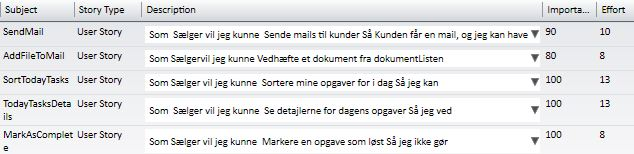
\includegraphics[width=1.00\textwidth]{Sprint4Backlog.jpg}
	\caption{Sprint 4 backlog}
	\label{fig:Sprint 4 backlog}
\end{figure}

\subsection{Burndown Chart}
Burndown chartet er blevet undladt da der slet ikke startet op p� dette sprint.

\subsection{Udf�relse af sprint 4}
I praktik perioden blev der lavet en metode til at sende automatisk e-mail til kunder der havde kontaktet kundeservice, s� implementeringen af selve afsendelsen af e-mail vil v�re en overskuelig opgave. Dertil kommer den synkronisering af e-mails som er blevet sendt til en kunde via Googles UI, f�r de er blevet oprettet i systemet som kunder. Selvf�lgelig ogs� efter hvis man skulle sende flere mails fra Google.

Udover sending af e-mails er UI lavet til TodayTask user stories, dog med noget dummy data, blot for at vise produkt owneren hvordan det ville komme til at se ud.

\section{Accept test}
Sidst i sprint tre ville vi gerne have haft vores produkt owner og en s�lger til at lave en r�kke Accept test som vi har skrevet. Form�let med disse tests er at f� produkt owneren til at teste om produktet lever op til hans krav. Der er ofte langt fra beskrivelserne i user stories til det brugerne rent faktisk mente. Ved hele tiden at have vist de nye metoder i vores sprint reviews burde der ikke v�re s� mange overraskelser p� den front. Det er mere funktionelle fejl, og test om brugerne kan finde ud af brugergr�nsefladen. Ud fra den respons vi ville have f�et kunne vi have planlagt vores fjerde sprint med de rettelser og eventuelle fejl der ville blive fundet ville finde. Vi vil starte med at teste nogle af systemets vigtigste funktioner. 

Vi n�ede desv�rre aldrig at f� sat vores accept test i gang. Vi ville gerne have lavet en bruger til de to testere, og s� egentlig bare s�tte dem foran systemet og lade dem k�re vores accept tests igennem. De skal selvf�lgelig tage noter omkring hvordan de oplever at bruge systemet. Samt skrive de fejl ned de oplever, og eventuelle m�der tingene kan g�res smartere for dem. 

Vi mener det er vigtigt at dem der rent faktisk skal bruge systemet er med til at teste det.

\subsection{Filter Leads}
Denne metode bruges til at filtre leads i oversigten. P� den m�de kan man finde frem til pr�cis de leads man �nsker at skulle arbejde med.

\begin{itemize}
\item G� ind p� Leads oversigt siden
\item Find alle Leads med post nummer mellem 9000 og 9400
\item Derefter filtre dem fra 
\end{itemize}

\subsection{Upload CSV}
Her kan man uploade en r�kke leads i en CSV fil. P� den m�de kan man oprette mange leads afgangen frem for et.

\begin{itemize}
\item G� in p� Leads oversigt siden
\item Upload udleveret CSV fil til systemet
\item V�lg de Leads blandt CSV-dubletterne der er rigtige
\item Godkend de valgte leads
\item V�lg de Leads blandt DB-dubletterne der er rigtige
\end{itemize}

\subsection{Find Lead Details og Kontakt Details}
Her finder vi detaljer omkring et bestemt lead og dens kontakter. 

\begin{itemize}
\item Sorter firmaerne s� kun Leads bliver vist i menuen til venstre
\item Find stamdata omkring leadet ved at klikke p� navnet
\item Find stamdata omkring en Kontakt fra leadet ved at klikke p� navnet i h�jre side
\item Find og l�s en note ved at kigge p� note historie
\item Opret en note omkring firmaet ved at klikke p� note knappen
\item Ret i firmaets stamdata ved at klikke i feltet der skal rettes
\end{itemize}

\chapter{Sikkerhed}

Eftersom det er en web-application er der altid nogle sikkerhedsaspekter forbundet med disse. Is�r hvis det er en siden som bliver lagt ud p� Internettet s� alle har adgang. Nu er vores kun til internt brug, s� vi forventer ikke der er nogen ondsindet brugere af vores system. Med det sagt har vi selvf�lgelig stadig gjort os nogle overvejelser omkring de mest basale sikkerhedshuller i webapplikationer. Vi mener det er et omr�de der skal tages seri�st, selvom de data vi arbejder med ikke er personf�lsomme b�r man stadig beskytte dem hvis man skulle v�re uheldig at f� de forkerte folk ind i virksomheden.

Et af de steder man ofte ser angreb p� hjemmesider er via SQL injections. Det er et angreb direkte p� de data man har i sin database, og derfor kan det v�re meget alvorligt hvis man kan f� adgang til disse. Man kan tr�kke data ud som man ikke normalt skal kunne se, eller man kan s�gar slette hele tabeller. 

Man udnytter de steder hvor brugeren skal taste oplysninger ind, da de input vil blive sendt videre til databasen. Dem manipulere man s� database tror det er en SQL kommando som den s� udf�re i stedet for at s�tte de data ind som man egentlig bad den om. Et simpelt eksempel kan v�re en login form, hvor bruger skal indtaste brugernavn og kode. Hvis det ikke er lavet ordenligt kan man kunne logge ind uden at kende passwordet. Hvis man skriver \verb| fakepassword' OR '1' | i password feltet vil databasen l�se det som at endte skal passwordet v�re "fakepassword eller ogs� skal "1" v�re true. Dermed har man s� f�et adgang da 1 vil blive opfattet som true. Alle de steder hvor man sender noget til databasen som brugeren kan manipulere p� en eller anden m�de skal man v�re opm�rksom p� denne type angreb.

Da vi bruger LINQ er der allerede taget h�nd om dette problem for os. LINQ bruger en klasse kaldet SQLParameter som s�rger for at vores input bliver lavet til parameter v�rdier, som uskadeligg�r denne type angreb. \citep{sqlinjection} Havde man bygget sine SQL-strenge op med almindelig SQL skulle man selv s�rge for disse parameter blev lavet for at undg� injections. 

Et andet typisk angreb p� web-sites er Cross-site scripting (XSS). Her kan man eksempelvis l�gge noget html eller JavaScript kode ind i databasen, hvorefter det s� bliver hentet ud igen og fortolket af browseren. Hvis man eksempelvis opretter en support-ticket i vores system, kan man tilf�je $<$b$>$ og $<$/b$>$ rundt om sin besked. Hvis man s� ikke tager h�jde for den slags vil browseren l�se det som at teksten skal st� med fed. Simpelt og harml�st, men det kan bruges til langt v�rre ting som at opsnappe personlige oplysninger osv. Da vi bruger Razor i vores views slipper vi nemt for den slags angreb da, de metoder vi bruger til at skrive tekst ud med har allerede taget h�jde for den slags, og skriver alt teksten ud, uden browseren fortolker noget af det. �nsker man at brugeren skal kunne formatere sine inputs kan man bruge HTML.Raw(), men s� er man igen s�rbar overfor XXS.

For at bruge vores system skal man have en bruger med login og password. N�r man har en bruger er en tilknyttet en eller flere titler. Det kan eksempelvis S�lger, Support eller Administrator. Ud fra disse titler og et sitemap over hele sitet kan vi styre hvilken omr�de hver bruger har adgang til. De steder hvor bruger ikke har adgang vil bruger typisk ikke kunne se linket der til, og skulle bruger skrive adressen manuelt vil han bliver flyttet v�k med en besked om adgang er n�gtet. 

For at logge ind har brugeren som sagt et brugernavn og password. Password har vi krypteret med en MD5 kryptering. Det er aldrig smart at gemme passwords i klar tekst. Ville man have yderligere beskyttelse her kunne man v�lge at salte sit password. Da vi ved det kun er til internt brug f�lte vi det var nok blot at kryptere passwordet. N�r man salter et password blander man et andet ord sammen med passwordet som s� bliver krypteret. P� den m�de bliver det endnu sv�rere at regne ud hvad passwordet i virkeligheden er, hvis man skulle f� fat i det.


\chapter{Perspektivering}
I dette afsnit vil vi evaluere p� forskellige omr�der i vores projektforl�b. Vi vil se p� hvad der er g�et godt og hvad der eventuelt kunne have v�ret gjort bedre og hvorfor.

\section{Roller og samarbejde}
Eftersom vi har benyttet os af Scrum som arbejdsmetode indebar det en r�kke rolle som skulle bes�ttes. Nogen af rollerne var selvskrevne mens andre er blevet taget ud fra et valg hvor vi mente vi fik mest ud af vores kompetencer. Roller blev inddelt som f�lgende. Martin Kristensen, Slagchef i EqualSums blev naturligt ProductOwner da han stod for kontakten til os. Peter Thomsen blev ScrumMaster, Gregers Boye-Jacobsen blev udvikler i ScrumTeamet. Scrum Masterens opgaver bestod prim�rt af at holde ScrumDesk opdateret og s�rge for vi s� godt som muligt fulgte den plan vi havde lagt og fik lavet tingene i den rigtige r�kkef�lge. De daglige Scrum m�der tog vi i f�llesskab med de �vrige medarbejdere hos EqualSums, hvilket bet�d vi p� den m�de hele tiden blev opdateret omkring hvad vi lavede. 

Udover Scrumroller har vi ogs� fors�gt at tage de arbejdsopgaver hvor vores kompetencer var h�jst. Gregers har blandt andet besk�ftiget sig mere med frontend end Peter, hvor Peter derimod har fokuseret mere p� backend koden. Det f�ler vi har virket utrolig godt, da vi begge prim�rt arbejder med det vi er gode til, og hvor vores prim�re interesse ogs� ligger. Det har ogs� betydet vi kunne n� at lave mere kode end hvis vi skulle sidde og k�mpe med noget den anden kunne klare p� langt kortere tid.

Dette var en arbejdsfordeling vi begge fandt helt naturlig under praktikperioden, s� det s� vi ingen grund til at �ndre. Det skal dog siges, at vi har lavet lidt af det hele, og v�ret rigtig gode til at tage tid til at hj�lpe og ikke mindst forklare og l�re fra os. Det er noget vi begge har haft stor gavn af. 

Derudover har vi haft en rigtig god �ben kommunikation, hvor vi hele tiden har f�et snakket mange forskellige ting igennem og diskuteret problemstillingerne godt igennem. Det f�ler vi i h�j grad har v�ret med til at h�jne produktets kvalitet og gjort, at de valg vi har truffet i hvert fald ikke er grebet ud af den bl� luft. 

N�r vi har kodet p� programmet har det n�sten kun v�ret ude p� EqualSums hvor vi har siddet ved siden af hinanden med hver sin computer. Det har derfor v�ret nemt for os hele tiden at sparre med hinanden, og hj�lpe hvis vi skulle sidde fast med et problem. Samtidig har vi ogs� haft mulighed for at sp�rge de andre 

Skrivearbejdet har vi fors�gt at dele ud dagen f�r, og er prim�rt blevet skrevet hjemme. Her har vi igen holdt kontakt med hinanden endte over MSN eller Skype. Vi har hele tiden fors�gt at holde en t�t kontakt, p� den m�de har vi fors�gt at g�re projektet til �t helt projekt selvom vi selvf�lgelig har arbejdet p� hver sine afsnit.

\section{Arbejdsmetode}
I vores metodeafsnit har vi som n�vnt valgt prim�rt at bruge Scrum, et f� XP og UP elementer. De scrum praksis vi har brugt har i h�j grad hjulpet os med at f� et st�rre overblik over projektet. Da man har stor �benhed i form af produktbacklogs og sprintbacklog har det v�re nemt for os at se hvem der laver hvad, og havde vi v�ret flere i gruppe er vi sikker p� dette ville have v�ret endnu tydeligere. Vi har dog savnet det at vi kunne h�nge vores backlogs op p� et whiteboard, da vi f�ler det giver endnu st�rre overblik. Dog har vi til geng�ld haft adgang til vores backlogs alle steder, da de ligger online i ScrumDesk. Det har vi is�r benyttet os af n�r vi har skrevet hjemme.

Vi har v�ret glade for at arbejde efter en agil arbejdsmetode da vi ofte l�bende har f�et sm� �ndringer fra kunden. Det ville have v�ret langt v�rre hvis vi havde lagt os mere fast i et design fra UP. 

De diagrammer vi har gjort brug af fra UP har hjulpet os hurtigere i gang, da de hurtigt giver et billede af hvilken retning projekt skal formes. Det giver os et godt fundament som vi kan l�ne os op af is�r i starten, for senere at bliver brugt mindre og mindre. Senere i forl�bet har vi tjekket op p� vores kode og diagram for at sikre at de stadig stemmer overens. Ellers har vi refactoret dem s� de passer med virkeligheden. 

De elementer vi har brugt fra XP f�ler vi i h�j grad har v�ret med til at �ge kvaliteten i programmet. Vi gjorde meget brug af at refactor vores eksisterende kode, og der er mange steder i koden hvor vi kunne forbedre metoder, og optimere stumper af vores program v�sentligt. Det er det af v�rkt�jerne fra XP vi har brugt mest. Derudover kunne vi godt t�nke os at lave det til et test drevent projekt, men der er bare en indl�ringskurve der gjorde vi ikke havde tid til i dette projekt.

Rent fysisk har vi siddet i samme lokaler som kunden og udviklet. Dette har v�ret en stor hj�lp, idet vi altid (op til konkursen) har kunne sp�rge, hvis der var ting vi �nskede at f� afklaret. Samtidig har kunden kunne se vores fremskridt, og stoppe os, hvis der var noget vi havde misforst�et.

Det har naturligvis h�mmet os, at virksomheden undervejs gik konkurs, da dette medf�rte, at vi ikke kunne bruge deres servere og database. Dette har betydet, at vi ikke har n�et at f�rdigg�re produktet. Vi er dog stadig tilfredse med det vi s� har n�et, og er glade for, at vi ikke valgte at skrive rapporten f�rst, og udvikle til sidst. 

Alt i alt har vi v�ret rigtig glade for den arbejdsmetode vi valgte i starten. Den har givet os en passende frihed, og samtidig sat nogle rammer op som hj�lper en med at strukturere projektet p� fornuftig vis. Vi f�ler den har v�ret med til at give os et bedre produkt og samtidig muligheden for at n� l�ngere.

\section{Produkt}
Som tidligere n�vnt, n�ede vi ikke at blive f�rdige med produktet. Dette var heller ikke meningen fra starten af, da vi ogs� skulle have tid til at skrive rapport. Kunden har dog v�ret indforst�et med dette, og vi har i udviklingsfasen gjort os store anstrengelser for, at det er nemt for en anden udvikler at overtage produktet. 

Med fare for at lyde som en konklusion fra folkeskolen, s� har det v�ret et sp�ndende produkt at udvikle. Vi har begge erfaring med webudvikling, men ikke mvc-frameworket. Der har derfor v�ret en del l�ring, men vi har ikke haft brug for at s�tte os ind i html, css og andre grundl�ggende web-teknikker. Dette har v�ret til stor gavn, og har betydet, at vi har kunne koncentrere os om alt det nye der skulle l�res ifbm. mvc-framework. Derudover var der ogs� en masse andre ting der skulle l�res som f.eks. LINQ og entity framework.
\chapter{Konklusion}

Vi skrev i problemformuleringen, at vi ville fokusere p� patterns der kunne hj�lpe med at l�se opgaven. Vi har i det forl�bne kigget p� repository, factory og decorator pattern, som vi har forklaret og implementeret. Der er brugt andre patterns i forl�bet, men disse er ikke blevet forklaret. Disse patterns er s� grundl�ggende, at vi vurderede, det ikke ville v�re relevant at g� i dybden med disse. 

Hvad ang�r de n�vnte patterns har de v�ret til stor hj�lp, og patterns er helt klart noget man som udvikler skal v�re opm�rksom p�, da man ellers risikerer at opfinde den dybe tallerken gang p� gang.

Samtidig er en anden konklusion, at en agil tilgang til projektet har v�ret den rigtige, da det har givet mulighed for, at kunden har kunne komme med input undervejs.

Skal der konkluderes p� selve produktet, m� konklusionen v�re, at MVC er et meget taknemmeligt framework der i mange henseender g�r en udviklers liv nemmere. Vi er overraskede over, hvor meget vi egentlig har f�et udviklet i forhold til den begr�nsede tid, og at vi kun har v�ret to mand om projektet, og der har v�ret relativt mange nye teknologier at s�tte sig ind i.

Mange af de valg vi har foretaget i starten mht. teknologier er kommet os til gode, da disse ogs� har gjort livet nemmere. 


\appendix
\newpage
\pagenumbering{Roman}

\chapter{Diagrammer}
Diagrammer kan findes p� den vedh�ftede cd sammen med kildekode og en elektronisk kopi af denne rapport.

%\addcontentsline{toc}{chapter}{Figurer}
%\listoffigures

\newpage
\addcontentsline{toc}{chapter}{Litteratur}
\bibliography{litteratur} %Inds�t navnet p� jeres BiBtEx fil her (Uden extension)
\bibliographystyle{plainnat}
\end{document}